\documentclass{article}

\usepackage{amsmath}
\usepackage{natbib}
\usepackage{graphicx}
\usepackage{siunitx}
\usepackage{float}
\usepackage{hyperref}
\newcommand\tab[1][1cm]{\hspace*{#1}}
\date{} 
\begin{document}





\begin{figure}[!tp]
\vspace{-10mm}

\includegraphics[scale=0.8]{ee.png}


\vfil
\hfil \Large \bf MIDDLE EAST TECHNICAL UNIVERSITY
 \hfil
\vfil

\vspace{5mm}
\vfil
\hfil \large \bf  EE462-464 COMMON PROJECT
 \hfil
\vfil
\begin{center}
\vspace{5mm}
\vfil
\hfil \large \bf Design of a SM-PMSM
Variable Frequency Drive with Matlab/Simulink \hfil
\vfil
\bf
\end{center}

\vspace{23mm}
Canberk DUMAN    \tab2030450


Mert ZEYBEK \tab\tab2167682


\vspace{5mm}
\small Date: 02/07/2020


\end{figure}

\newpage

\section*{Introduction}
\tab Surface Mount Permanent Magnet Synchronous Machines are very popular in many applications. They are especially useful when precise speed and position control is required. In this project, Surface Mount PMSM drive is simulated using two different Pulse With Modulation techniques. \\
\tab Firstly, pre-design parameters are calculated according to machine parameters. After that Sinusoidal and Space Vector PWM methods are applied. Responses of electric drive under different circumstances such as change in the load torque, change in the speed reference are observed for both models. According to results obtained from these parts, two techniques are compared in terms of their THDs and suitability for high performance drive.
\section{Pre-Design Stage}
\textbf{1-} Rated torque is calculated as below considering $P_{nominal}$ and $n_{nominal}$:
\begin{equation}
    T_{rated}=\frac{P_{nominal}}{n_{nominal}}=\frac{400*10^3}{2 \pi*\frac{1500}{60}}=2546.49 Nm
\end{equation}
\textbf{2-} For the maximum electrical frequency, $n_{max}$ is used, which is 2250 rpm. Maximum electrical frequency is calculated below:
\begin{equation}
    f_{max}=\frac{n_{max}p}{120}=\frac{2250*4}{120}=75 Hz
\end{equation}
According to that, switching frequency is selected as 5 kHz for SVPWM, which is high enough for maximum frequency.
\textbf{3-} For the DC link of the rectifier, $1 mF$ capacitor is used. Braking resistance is selected as $0.18 Ohms$, which was ensuring that DC link voltage does not exceed 600 V, when the speed reference is reversed in the following stages. With the triangular block, hysteresis control is implemented in order to control DC voltage with IGBT. Picture of the model used for obtaining DC link voltage is given below:
\begin{figure}[H]
    \centering
    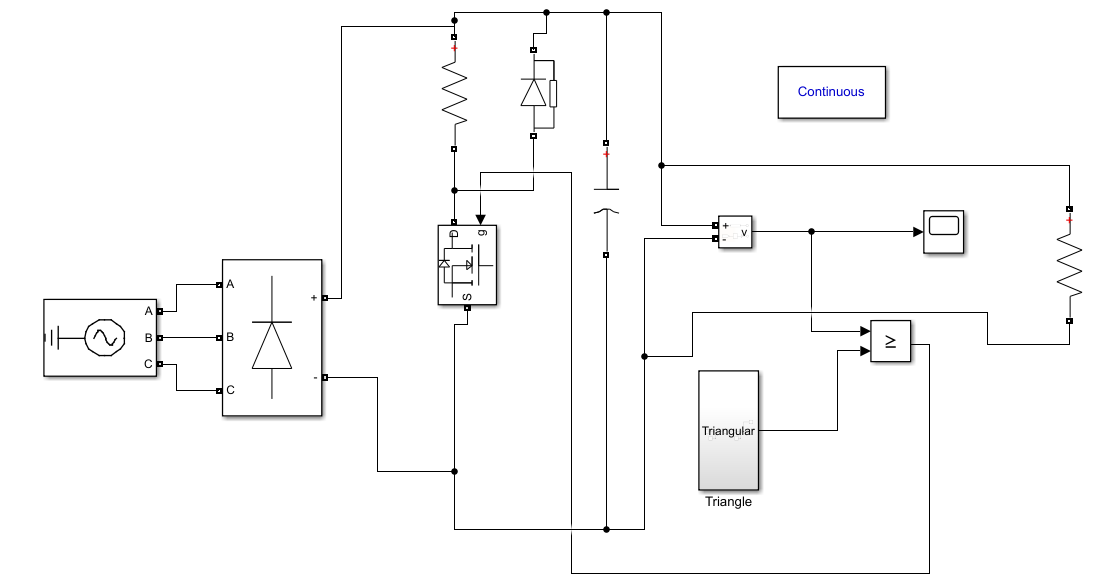
\includegraphics[scale=0.4]{r_load.PNG}
    \caption{DC Link Voltage Measurement Simulink Model}
    \label{fig:my_label}
\end{figure}
Voltage waveform obtained from the model is also provided below:
\begin{figure}[H]
    \centering
    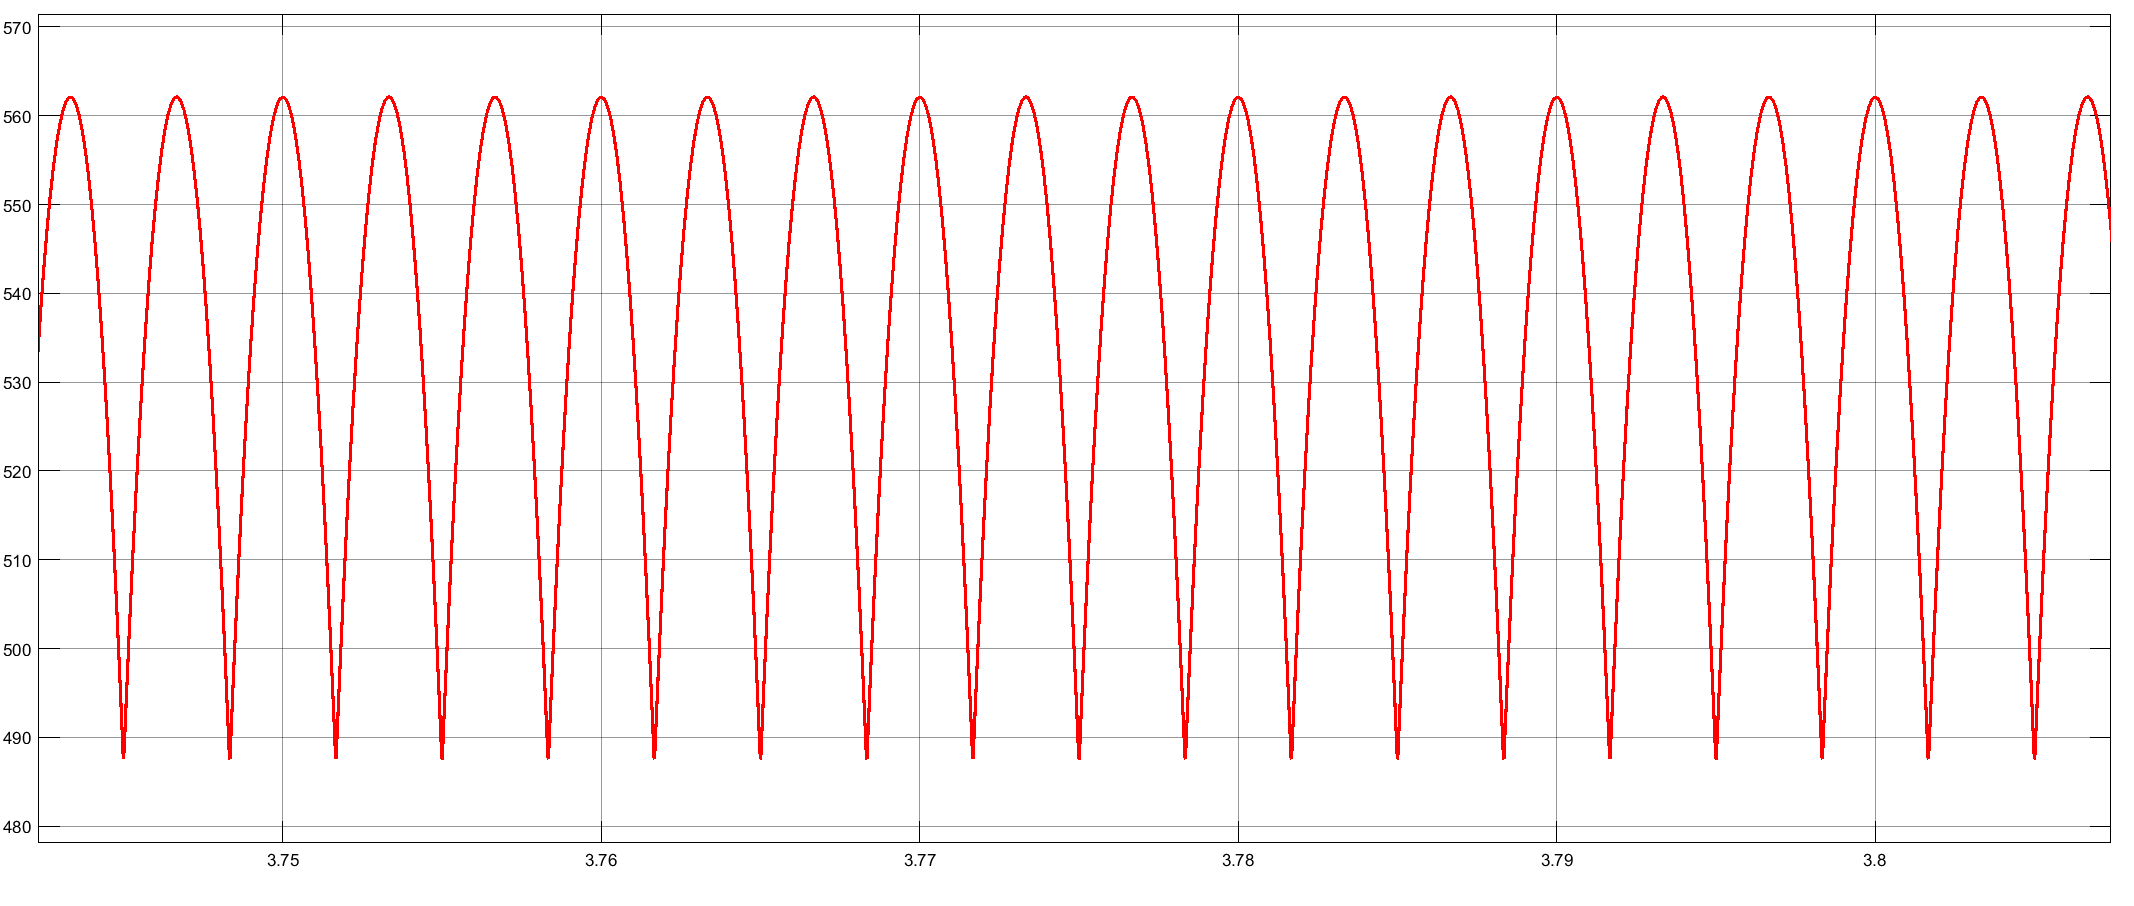
\includegraphics[scale=0.2]{dc_link.png}
    \caption{DC Link Voltage Waveform}
    \label{fig:my_label}
\end{figure}
\tab DC link voltage for 3-phase diode rectifier can be calculated analytically as below:
\begin{equation}
    V_{dc}=\frac{3\sqrt{6}}{\pi}V_{rms}=\frac{3 \sqrt{6}*230}{\pi} \approx 540 V
\end{equation}

\section{Sinusoidal PWM}
\section{Space Vector PWM}
\tab For the Space Vector PWM model, line currents of the motor, angular speed and position of the rotor of the motor are measured. These measurements are used in feedback implementation. In addition to that, $I_d$ and $I_q$ currents and $T_e$  are also measured in order to verify results. Line currents are transformed into $I_{alpha}$ and $I_{beta}$ by using created Clark Transform subsystem. $I_{alpha}$ and $I_{beta}$ are transformed to $I_d$ and $I_q$ using Park Transform subsystem and electrical angle of the rotor. This $I_q$ is compared with output of PI controller, which is controlling difference of measured speed and speed reference. $2/3$ gain is added to output of the speed controlling PI controller, which comes from power invariant transformation, flux linkage of magnets and pole pair number. With using another PI controller, we managed to acquire or desired $V_q$ voltage. \\
\tab To determine $V_d$ voltage, $I_d$ value is compared with 0, since we do not desire any d-axis current in the base speed region. Output of PI controller in this stage gave us $V_d$ voltage. \\
\tab By using inverse Park transform block, $V_{alpha}$ and $V_{beta}$ are acquired. These signals are given as input to SVPWM generator block, whose output was connected to Universal Bridge's gate signal input. Picture of the complete model for SVPWM simulation is given below:
\begin{figure}[H]
    \centering
    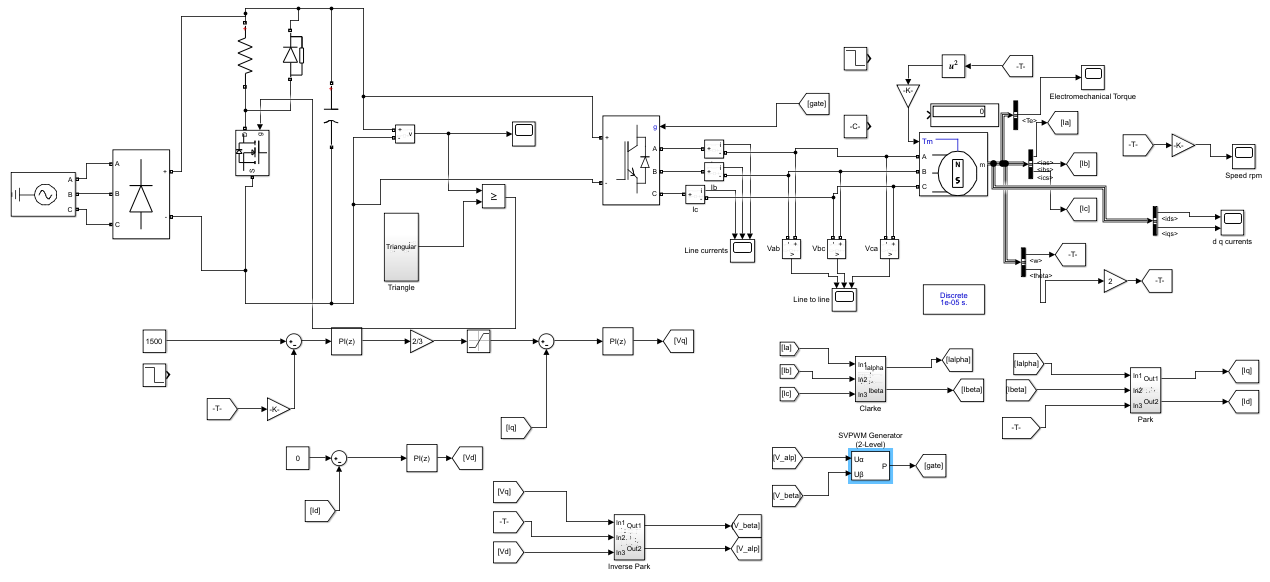
\includegraphics[scale=0.4]{svpwm_simulink.PNG}
    \caption{SVPWM Simulink Model}
    \label{fig:my_label}
\end{figure}
\textbf{1.1-} When the SM-PMSM is driving the fan load with $T_{load}=0.09 \omega $ and $J=240 kg m^2$ load, starting from $90 \% $ the nominal speed with SVPWM technique, following results are observed. At first, motor started from 1350 rpm and its speed increased linearly until it gets close enough to speed reference, which is 1500 rpm. In this case, motor reached its steady state at 1498 rpm, which is close enough to rated value. \\
\tab Motor created a high torque which is around 2560 Nm, in order to accelerate the load. Generated torque remained constant, until the machine reaches steady state at which load torque and generated torque are equal. At this stage, torque decreased slightly. \\
\tab $I_d$ oscillated around 0 A as expected. $I_q$ was 1700 A before the system reaches stead state. After that, it reduced to 1500 A, proportional to generated torque. Obtained waveforms are given below:
\textbf{a)}
\begin{figure}[H]
    \centering
    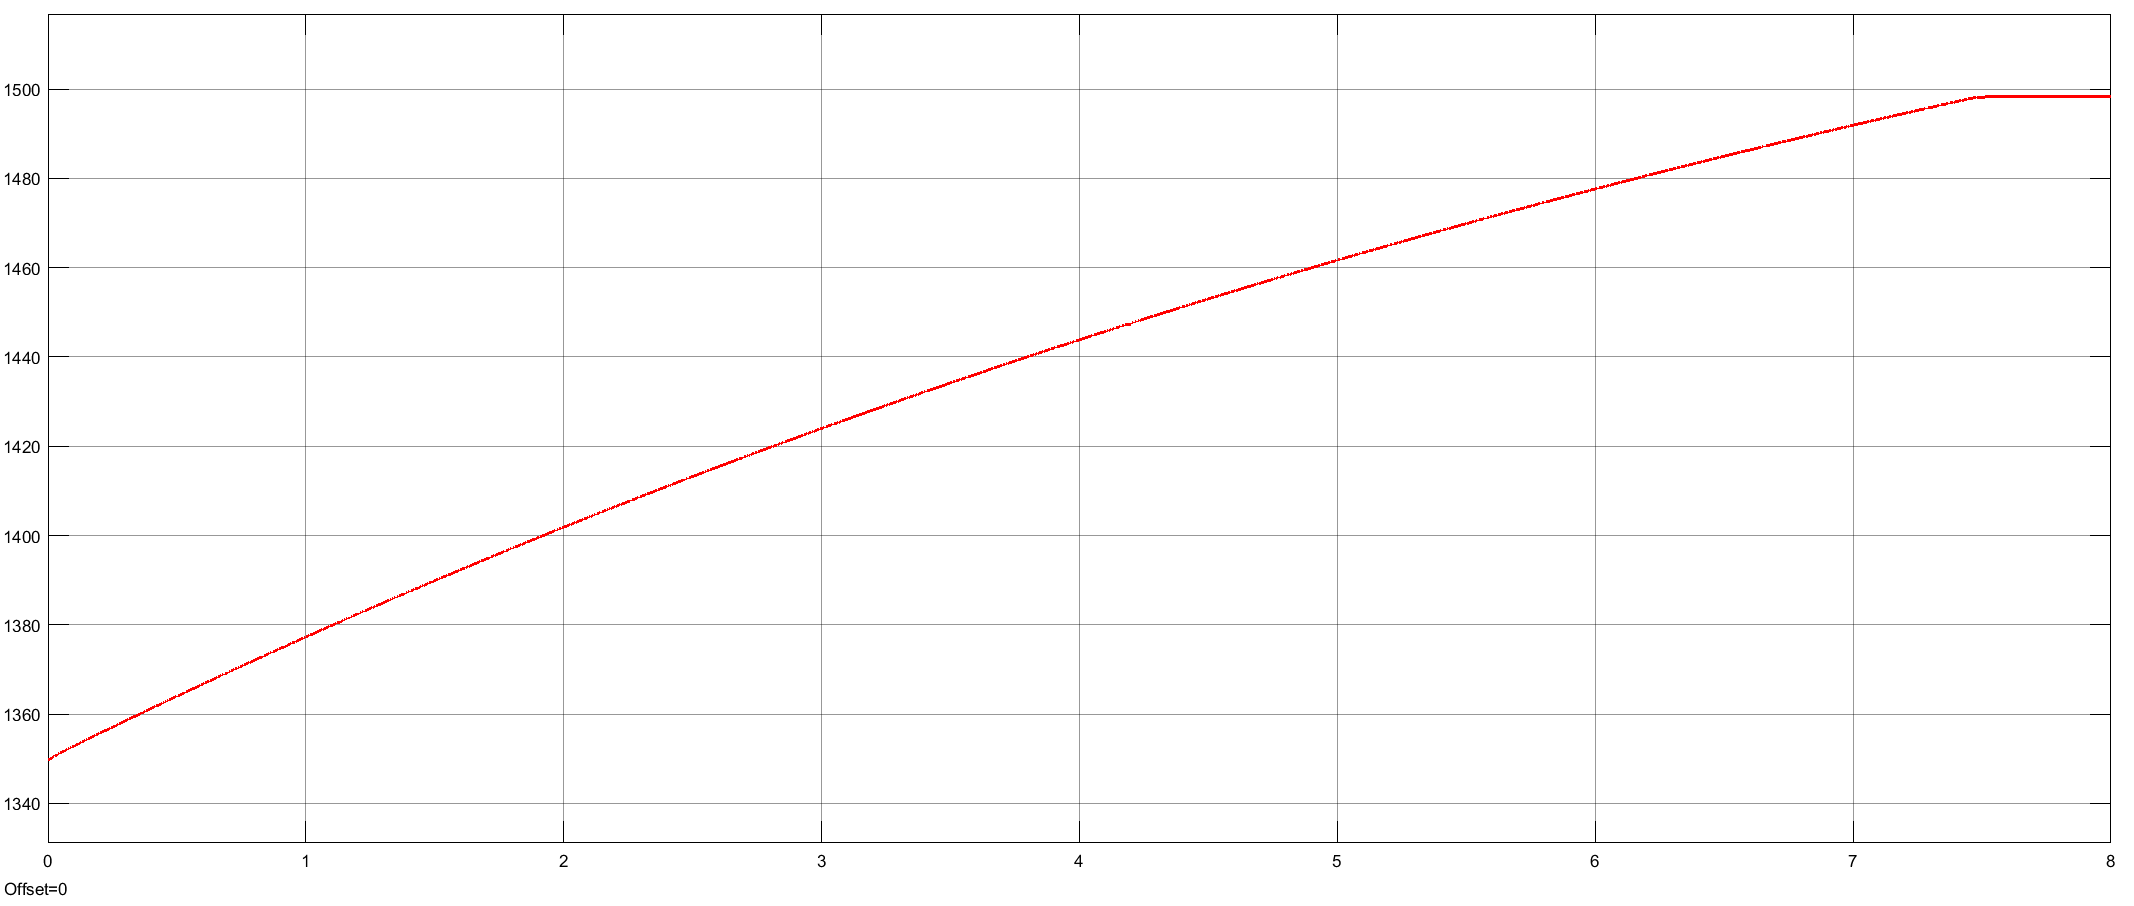
\includegraphics[scale=0.2]{q1a.png}
    \caption{Acceleration of SM-PMSM with Fan Load from 90 \% Rated Speed }
    \label{fig:my_label}
\end{figure}
\newpage
\textbf{b)}
\begin{figure}[H]
    \centering
    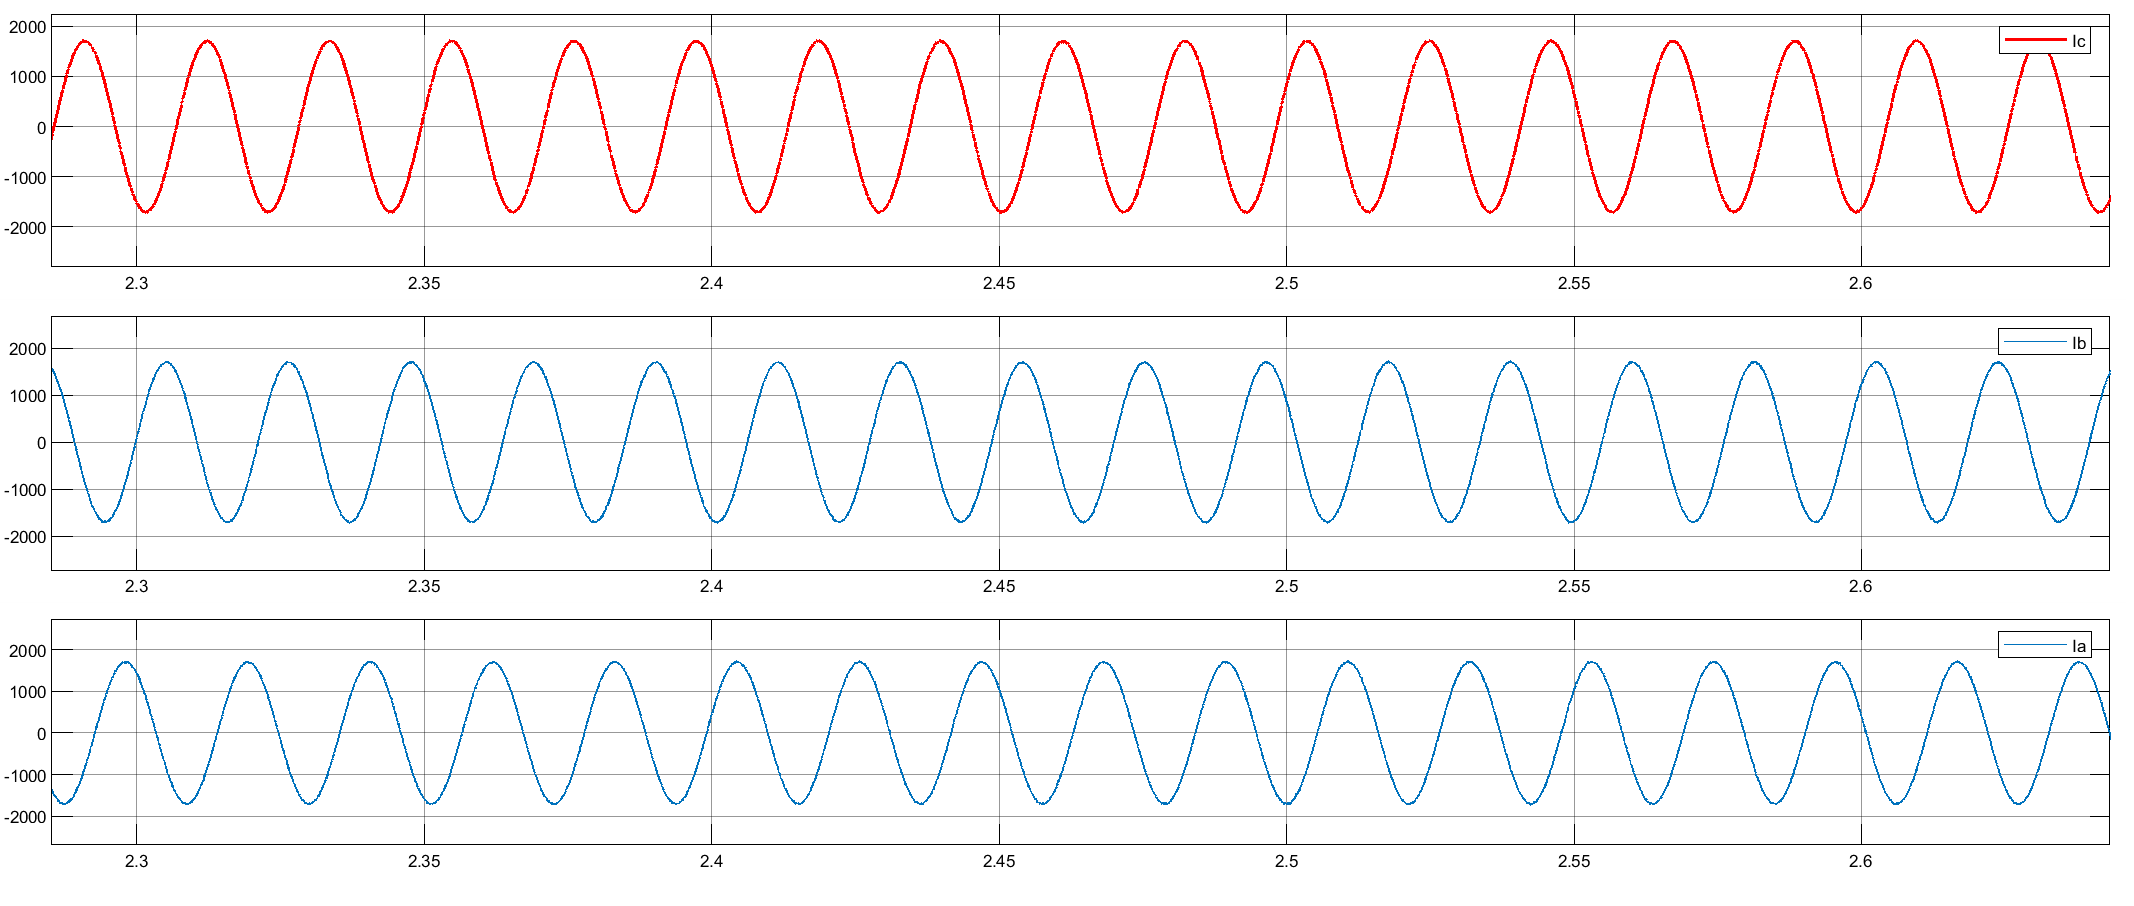
\includegraphics[scale=0.2]{q1_line currents.png}
    \caption{Graph of Line Currents During Acceleration of Fan Load}
    \label{fig:my_label}
\end{figure}

\begin{figure}[H]
    \centering
    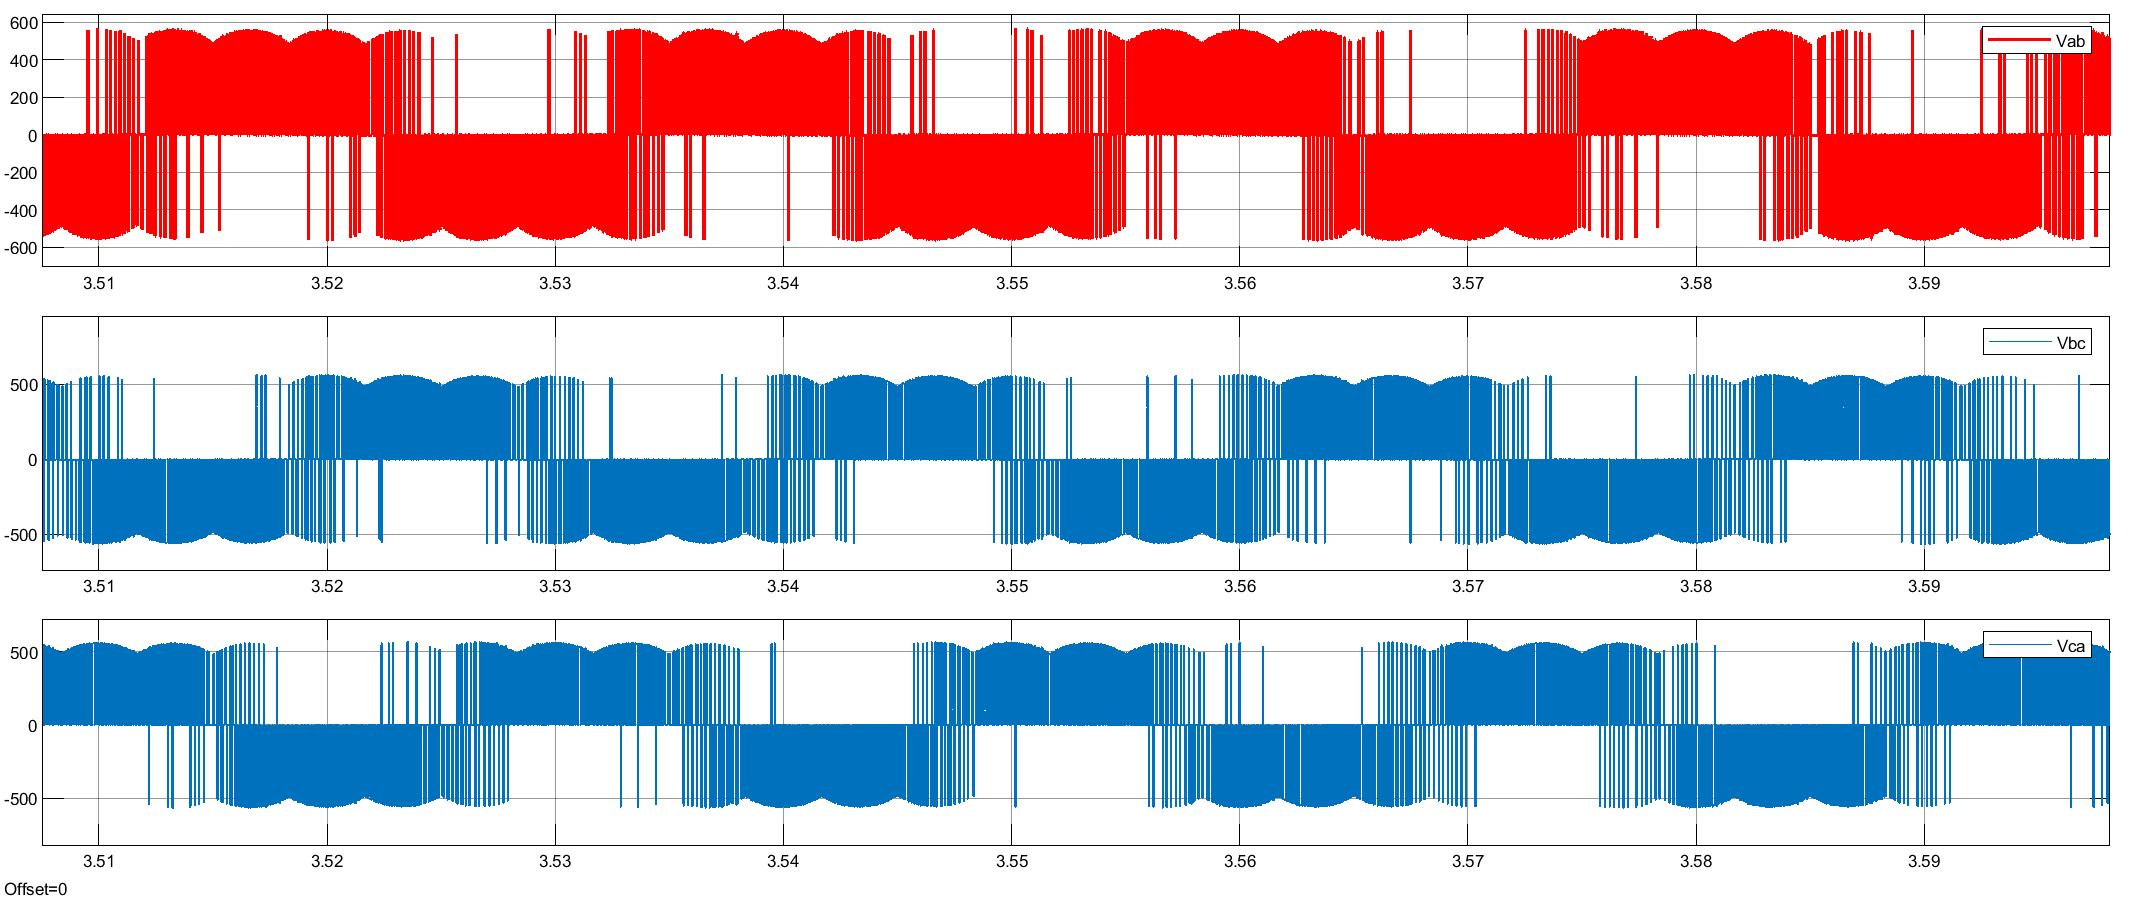
\includegraphics[scale=0.2]{q1_volts.png}
    \caption{Graph of Line to Line Voltages During Acceleration of Fan Load }
    \label{fig:my_label}
\end{figure} \newpage
\textbf{c)}
\begin{figure}[H]
    \centering
    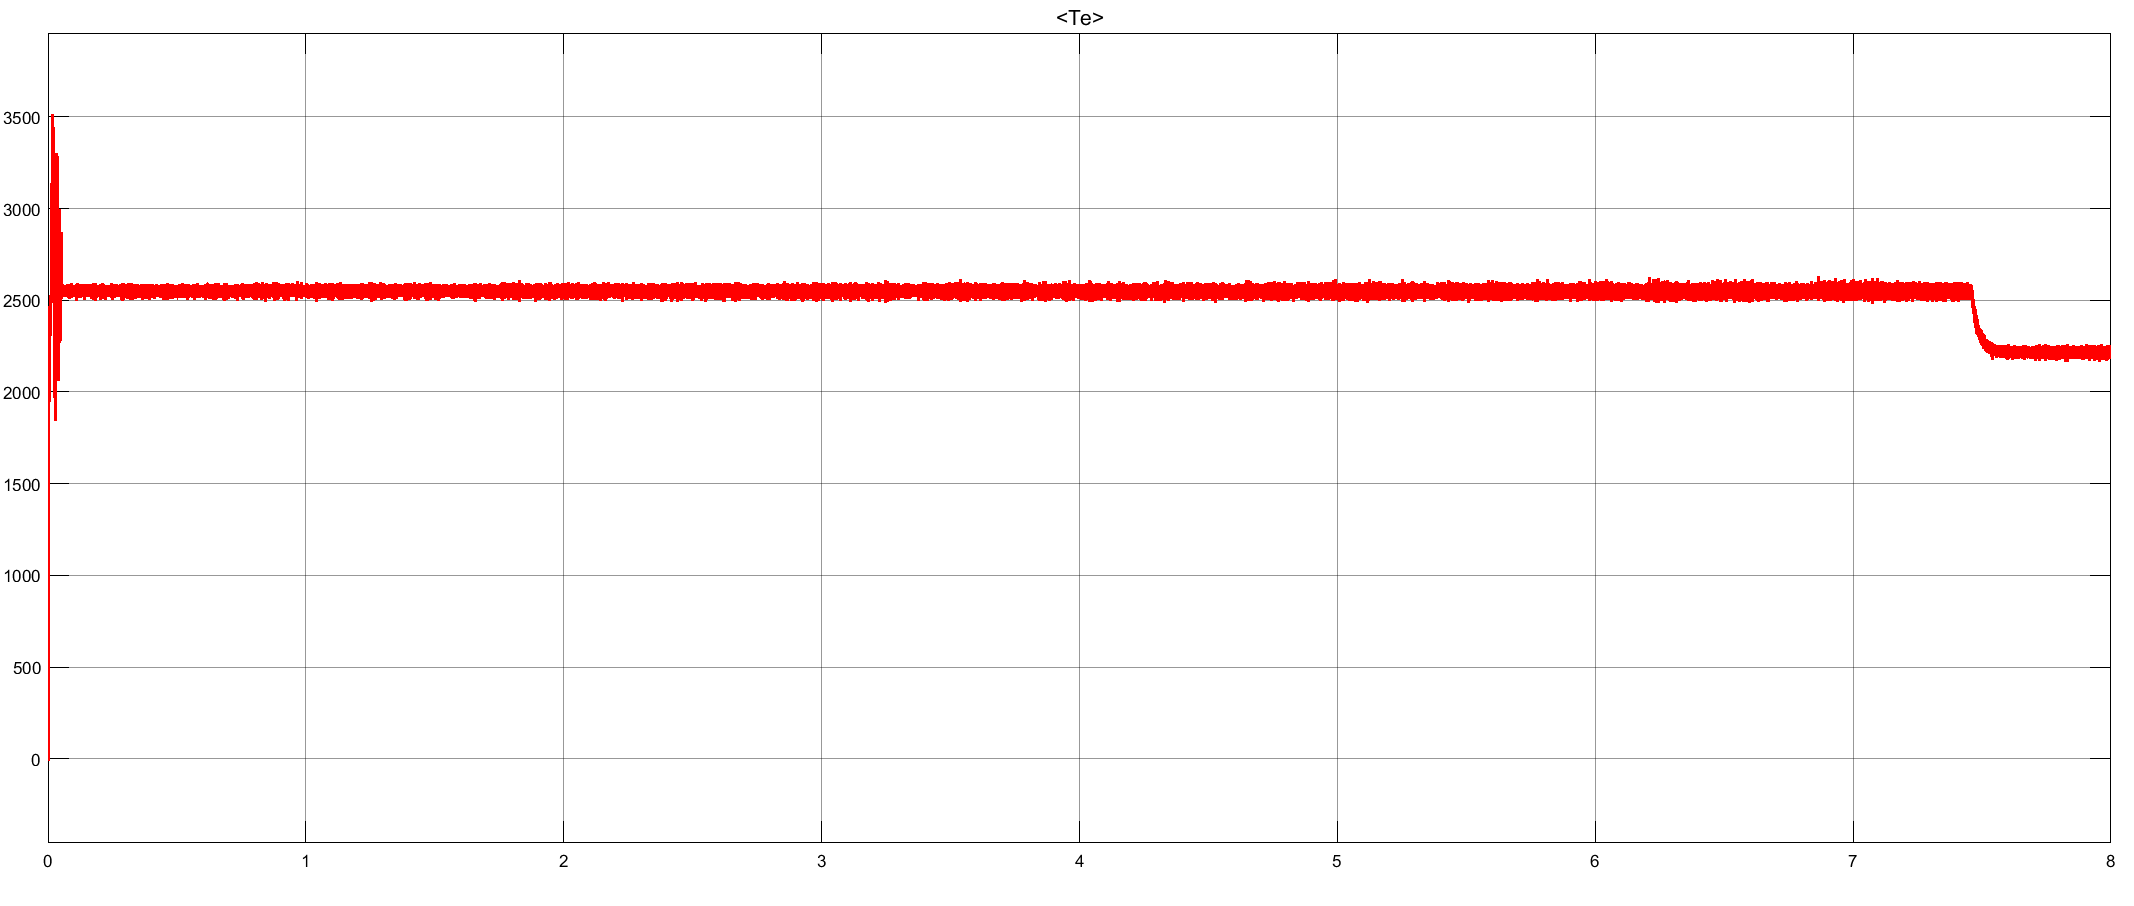
\includegraphics[scale=0.2]{q1_torque.png}
    \caption{Graph of Electromechanical Torque During Acceleration of Fan Load }
    \label{fig:my_label}
\end{figure}
\textbf{d)}
\begin{figure}[H]
    \centering
    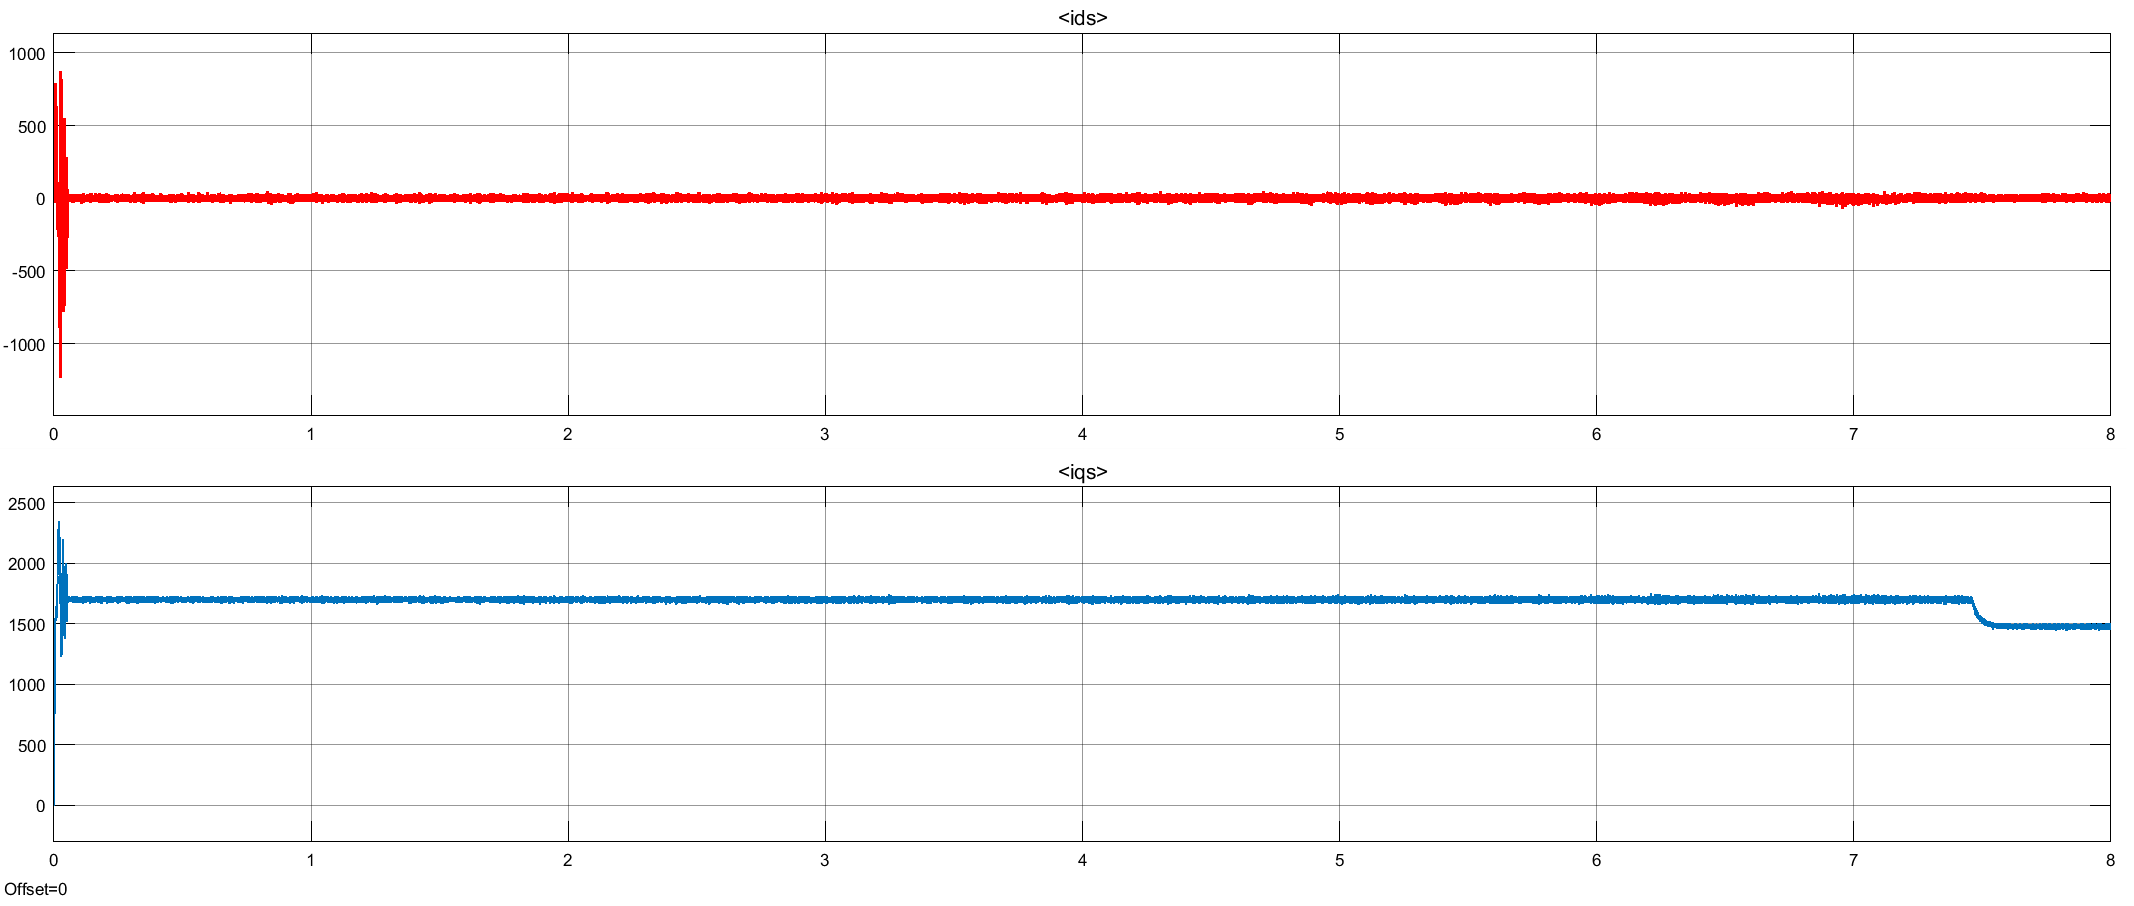
\includegraphics[scale=0.2]{q1_dq.png}
    \caption{Graph of $I_d$ and $I_q$ During Acceleration of Fan Load }
    \label{fig:my_label}
\end{figure}
\textbf{e)} Transition from $90 \%$ speed to rated speed takes 7.45 seconds. \\
\newline \textbf{1.2-} In order to model the change in the load torque, step function is applied to torque input of the machine. Initial value of step function is selected as 2214 Nm, which is the load torque at steady state rated speed. Since the load is removed when the load torque drops to zero, total inertia of the rotor is reduced from $250 kg m^2$ to $10 kg m^2$, since there is only rotor's inertia when the system is not at the steady state. Since the inertia is lower than the actual value before the removal of the load, there is some oscillation before the removal, which would not happen in the real case.\\
\tab The speed initially increased when the load is removed since generated torque accelerates the machine. After that, machine generated negative torque values in order to decelerate and reach speed reference, which indicates that machine got into generating mode for short amount of times. Torque and speed continue to oscillate as a result, with speed reaching to zero. However, for high inertia values, system remains stable and can reach back to its reference speed. Waveforms for the removal of the load case are given below:
\begin{figure}[H]
    \centering
    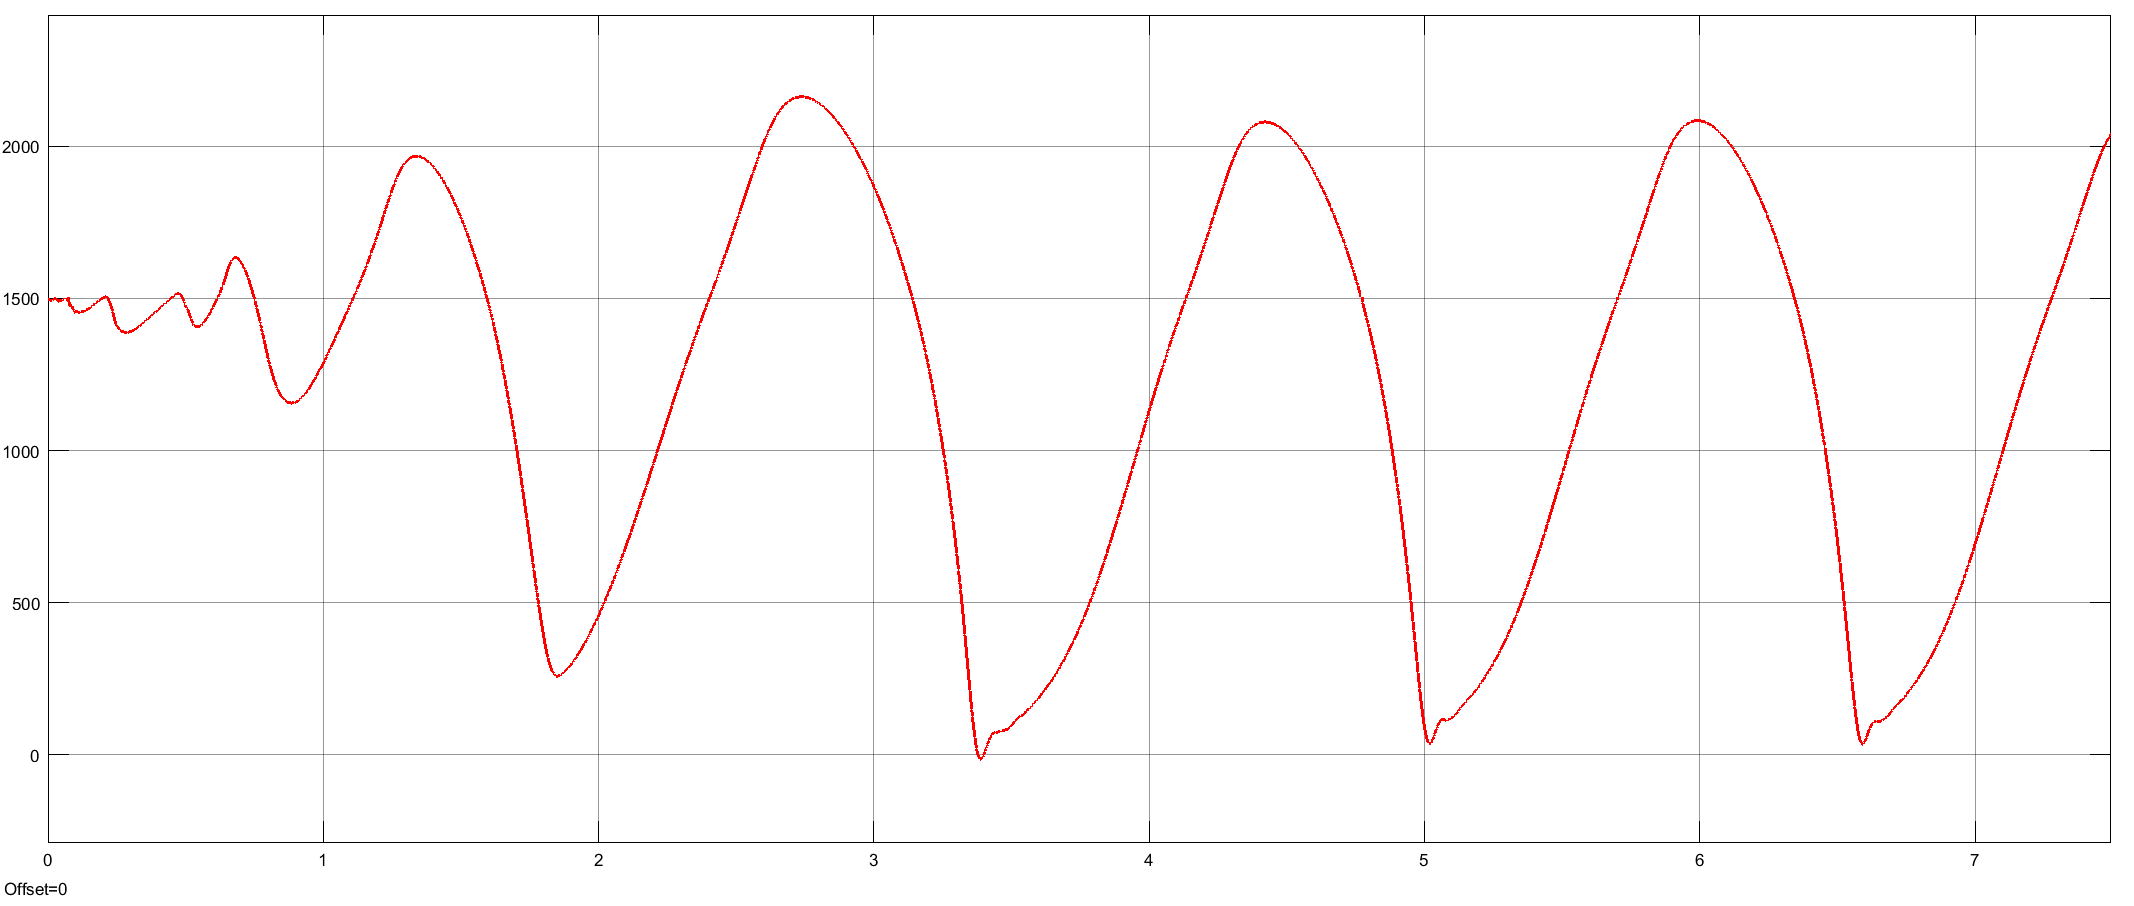
\includegraphics[scale=0.2]{q2_speed.png}
    \caption{Speed of SM-PMSM Rotor when the Fan Load is Removed }
    \label{fig:my_label}
\end{figure}

\begin{figure}[H]
    \centering
    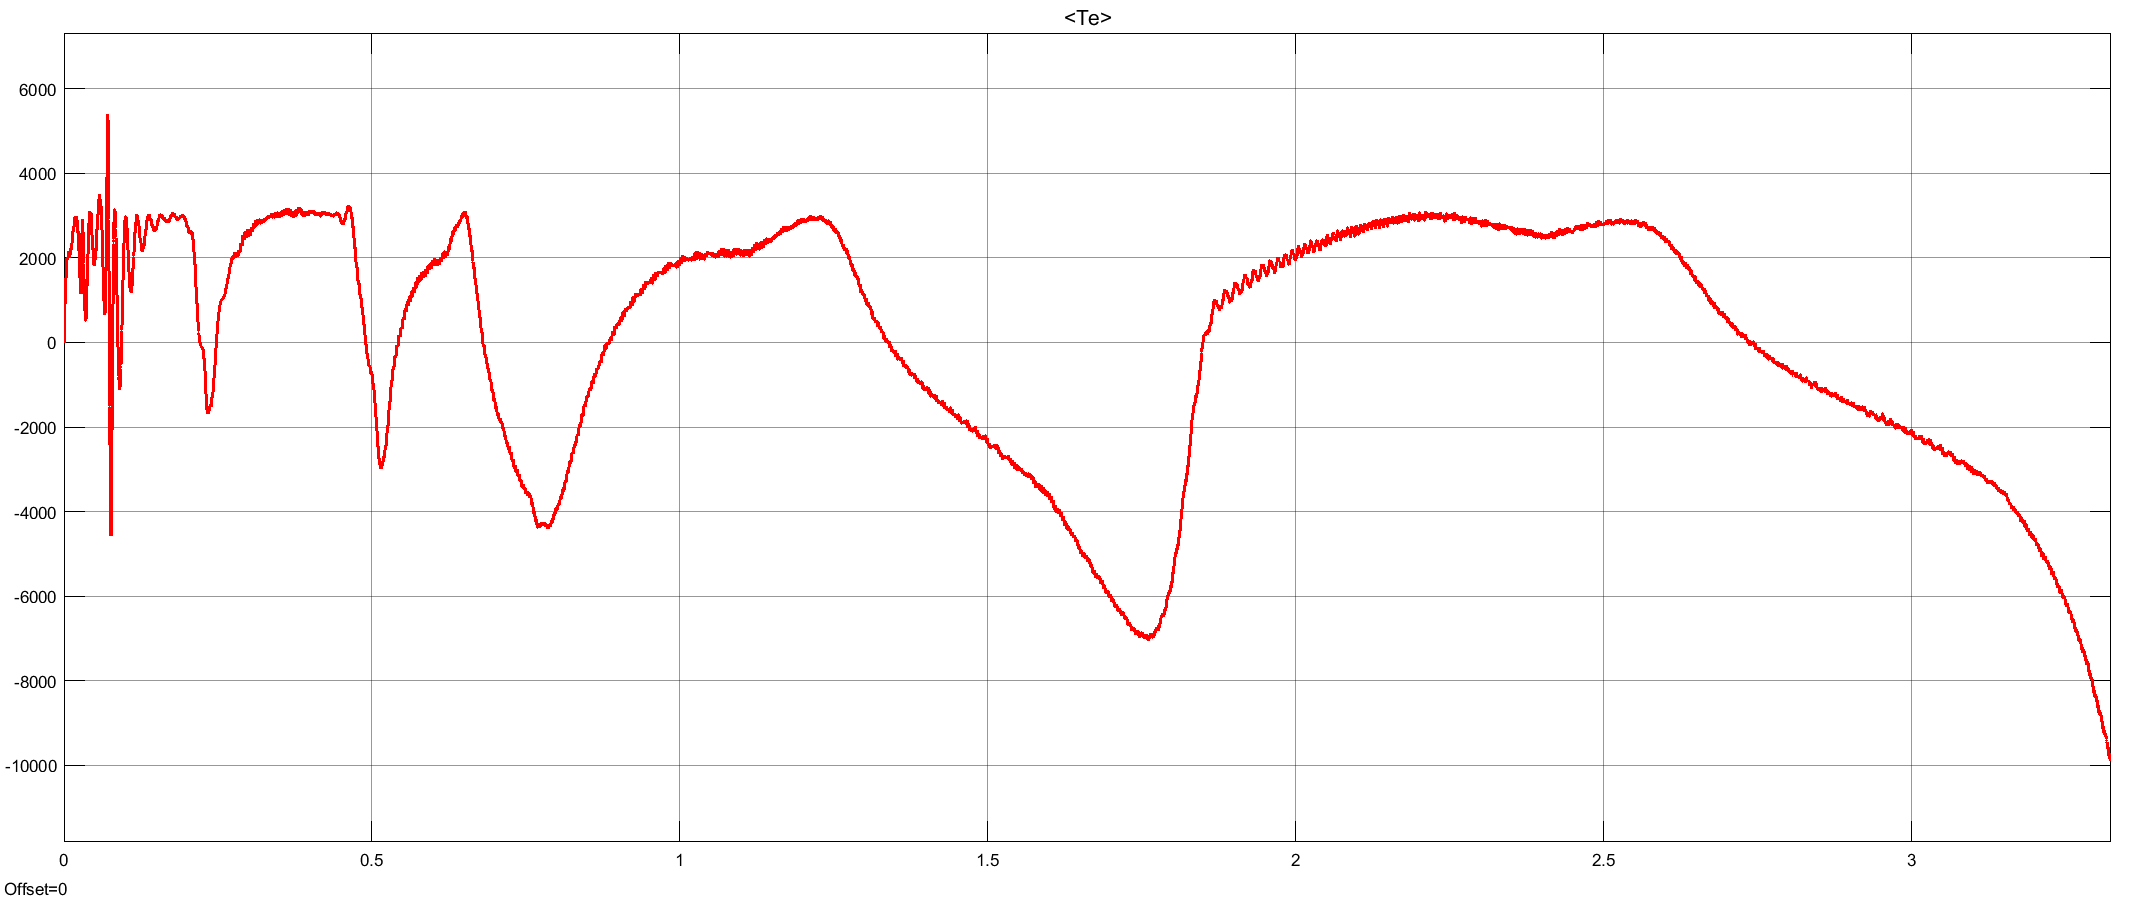
\includegraphics[scale=0.2]{q2_torque.png}
    \caption{Torque of SM-PMSM Rotor when the Fan Load is Removed }
    \label{fig:my_label}
\end{figure}

\begin{figure}[H]
    \centering
    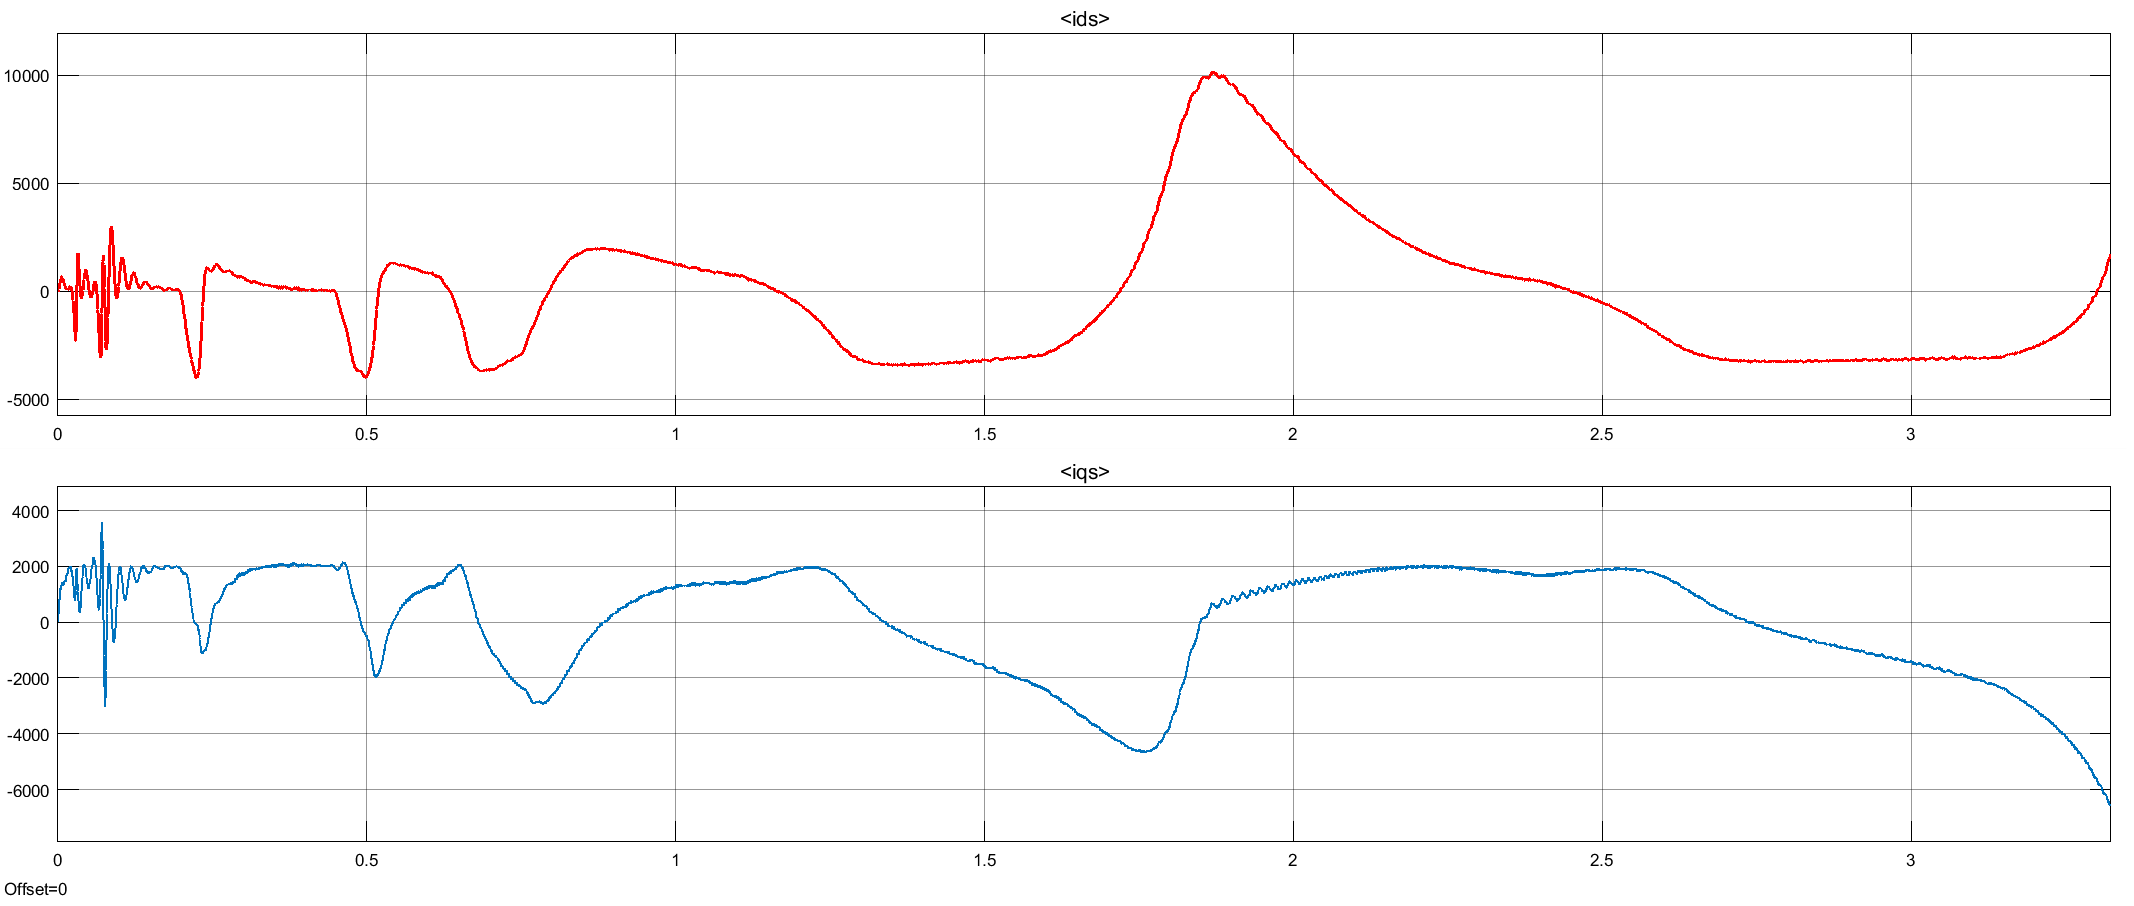
\includegraphics[scale=0.2]{q2_dq currents.png}
    \caption{Graph of $I_d$ and $I_q$ when the Fan Load is Removed }
    \label{fig:my_label}
\end{figure} \\
\newline \textbf{1.3-} To model reversal of the speed reference, step function is again used with 1500 and -1500 rpm values. There were no load inputs given for the machine. The torque is initially at zero as expected since there is no loss or load in the system. When the speed reference is changed, it generates a negative torque since it gets into generating mode. After that, negative torque value decreases and remains for some time which enables machine to accelerate linearly in the negative direction. Once the system reaches steady state once again in the -1500 rpm, torque value goes back to zero. $I_d$ current remains to oscillate around 0 A once again considering there is no field weakening. However, its oscillation increases at the reversal moment. $I_q$ current graph is similar with the torque graph since it is the current that creates the torque. \\
\tab Since the machine gets into generating mode, DC link voltage increases at the reversal moment. To limit DC link voltage, braking resistor is needed. when we use 0.18 Ohms braking resistance, maximum value of DC link voltage is 592 V, which is below the limit. Although we can manage to keep DC link voltage below the limit, the energy is converted to heat and efficiency is reduced. Instead of unipolar switches (diodes) in the rectifier topology, using unipolar switches would allow us to send generated power back to the grid. Efficiency would increase and there would be no need for the braking resistance. Hence, we can say that diodes are not feasible for this operation. Obtained graphs for this scenario are given below: \\
\textbf{a)}
\begin{figure}[H]
    \centering
    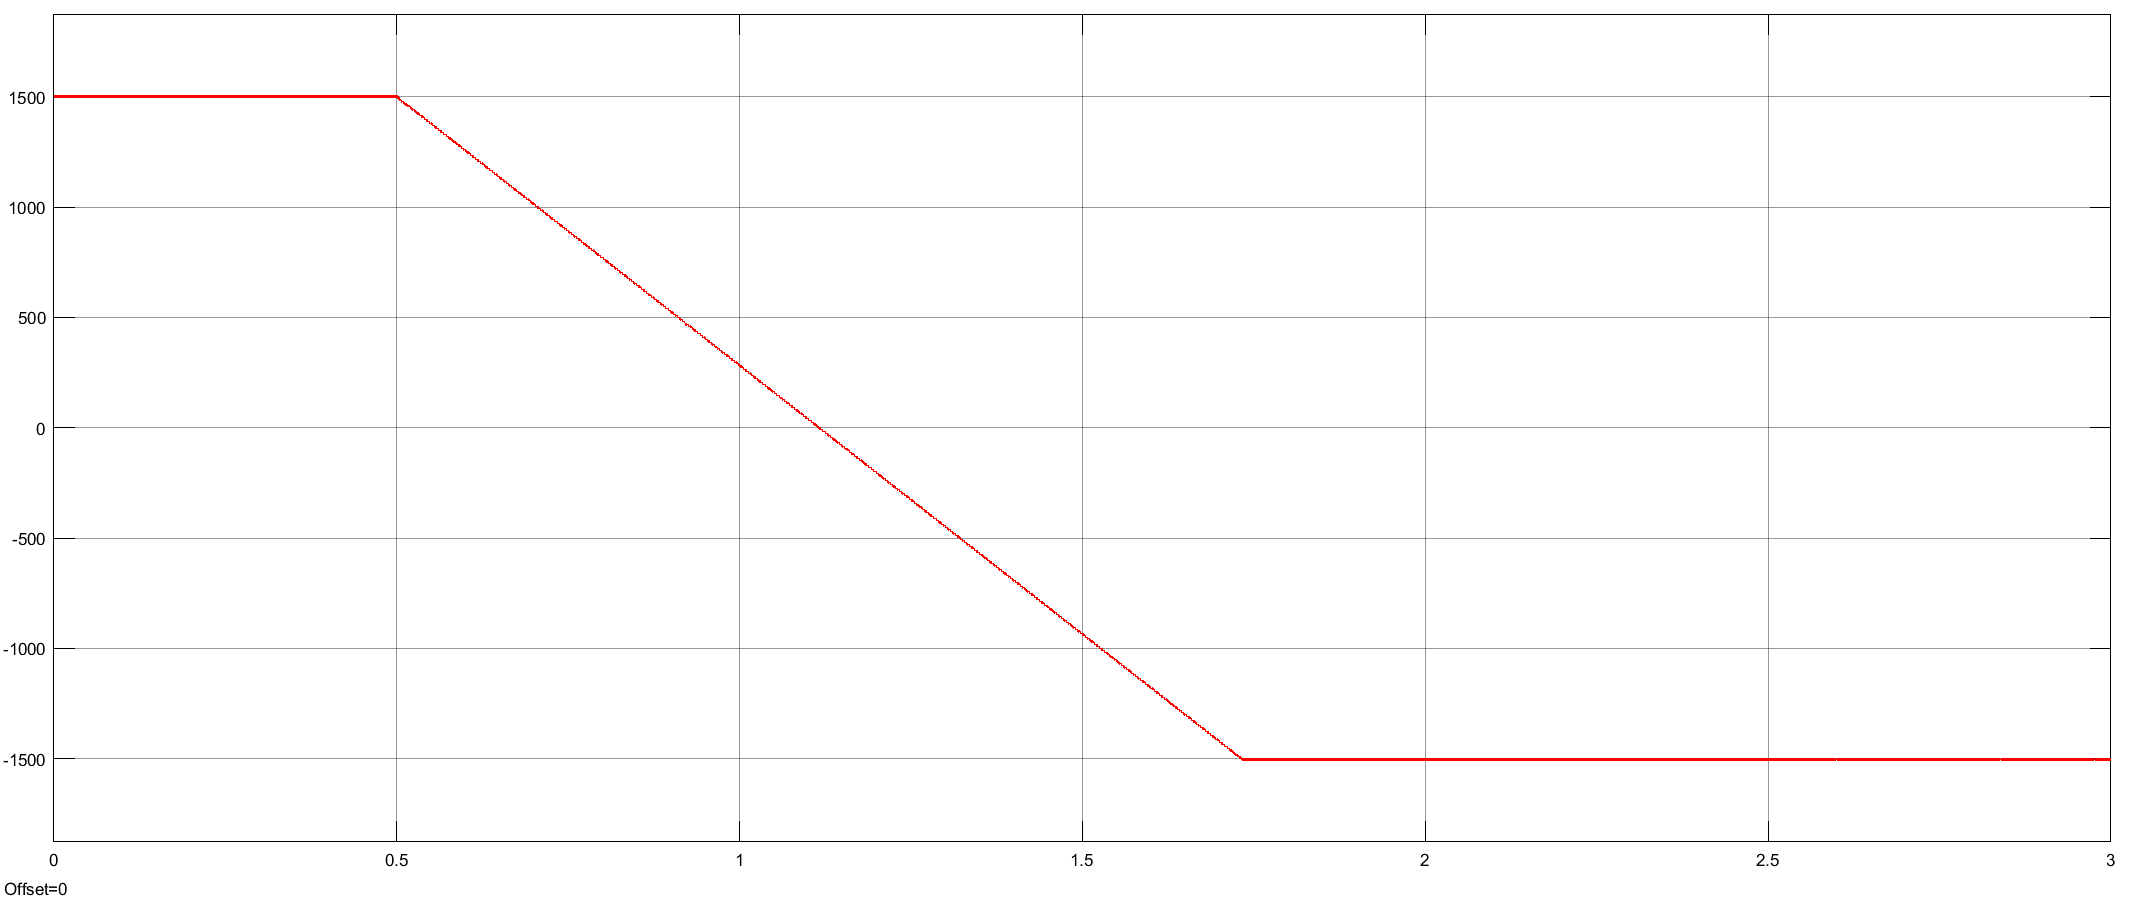
\includegraphics[scale=0.2]{q3_speed.png}
    \caption{Speed of SM-PMSM Rotor when Speed Reference is Reversed}
    \label{fig:my_label}
\end{figure}
\newpage
\textbf{b)}
\begin{figure}[H]
    \centering
    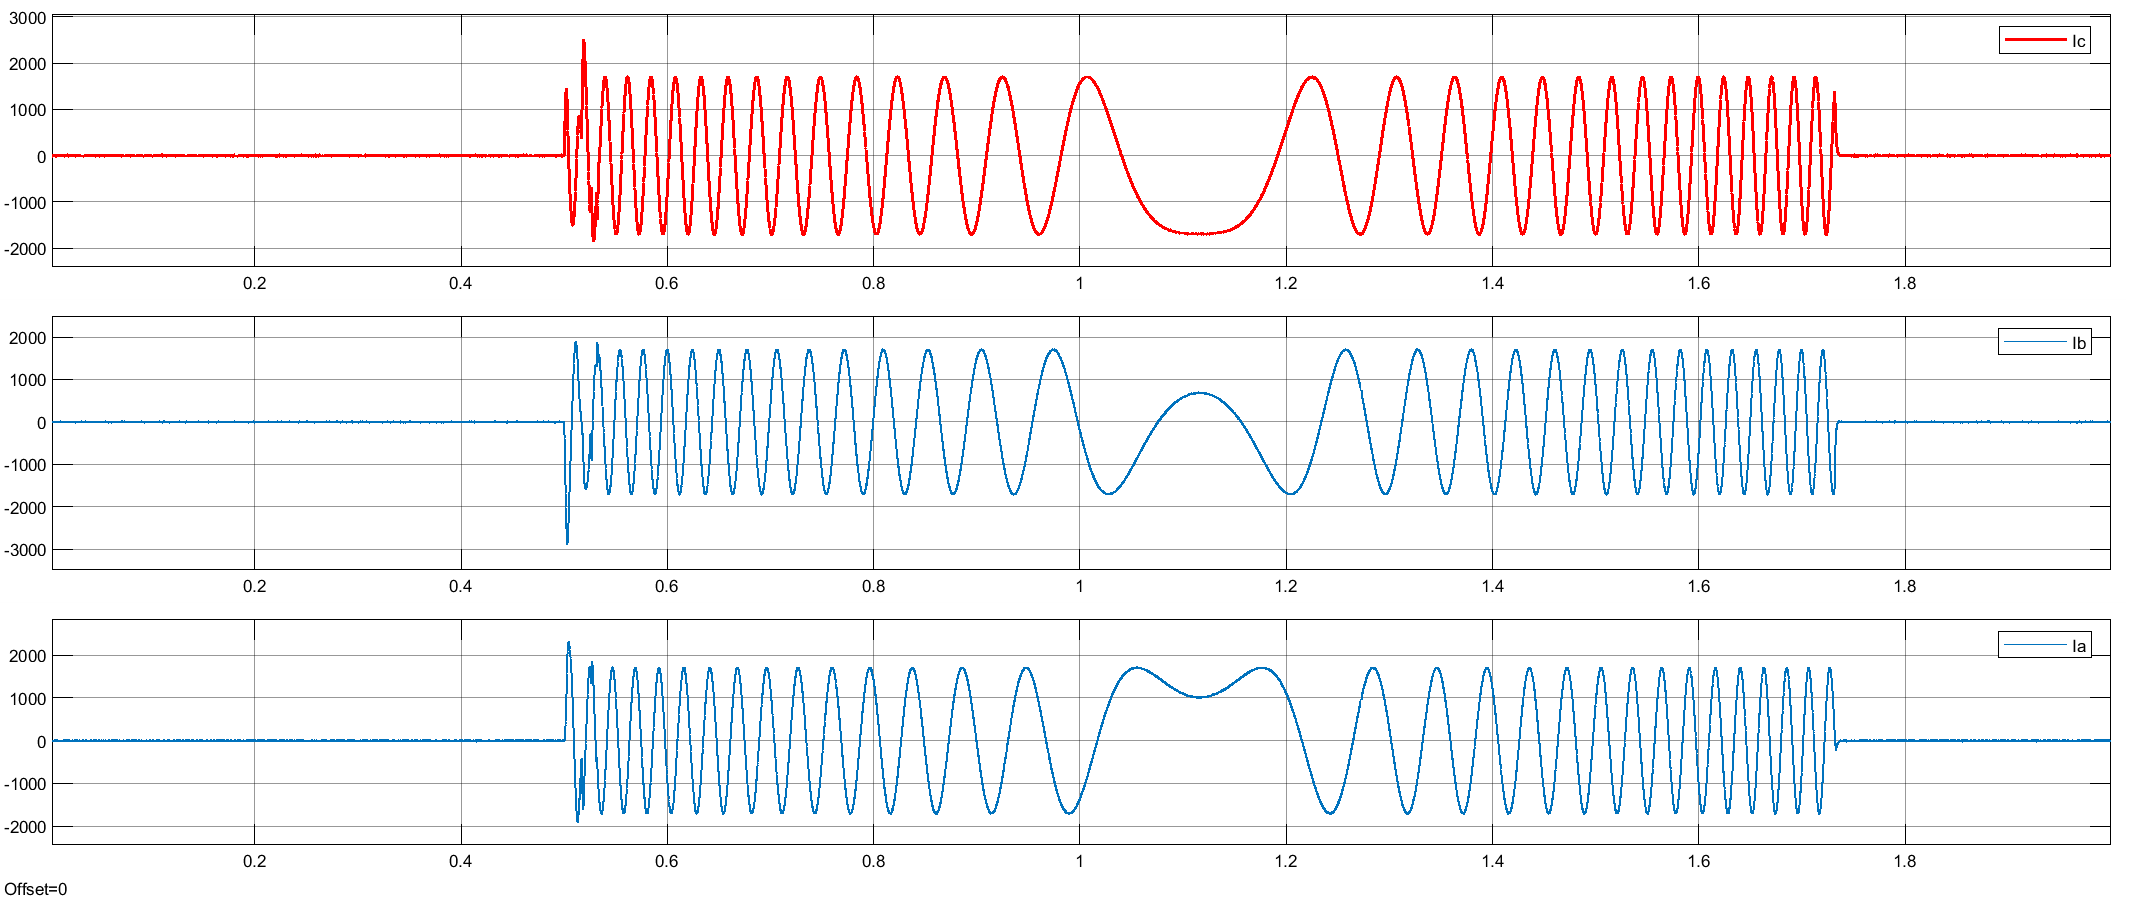
\includegraphics[scale=0.2]{q3_line currents.png}
    \caption{Graph of Line Currents when Speed Reference is Reversed}
    \label{fig:my_label}
\end{figure}
Line currents are zero at the 1500 and -1500 rpm steady states since we draw no power from the inverter at these cases as expected. At first, machine's speed decreases, which also decreases frequency of the line currents. When the mechanical speed reaches 0, line currents frequency is also minimum, which is around 1.12 seconds in the graph. After that, mechanical speed increases once again, increasing electrical frequency and frequency of the line currents.  \\
\textbf{c)}
\begin{figure}[H]
    \centering
    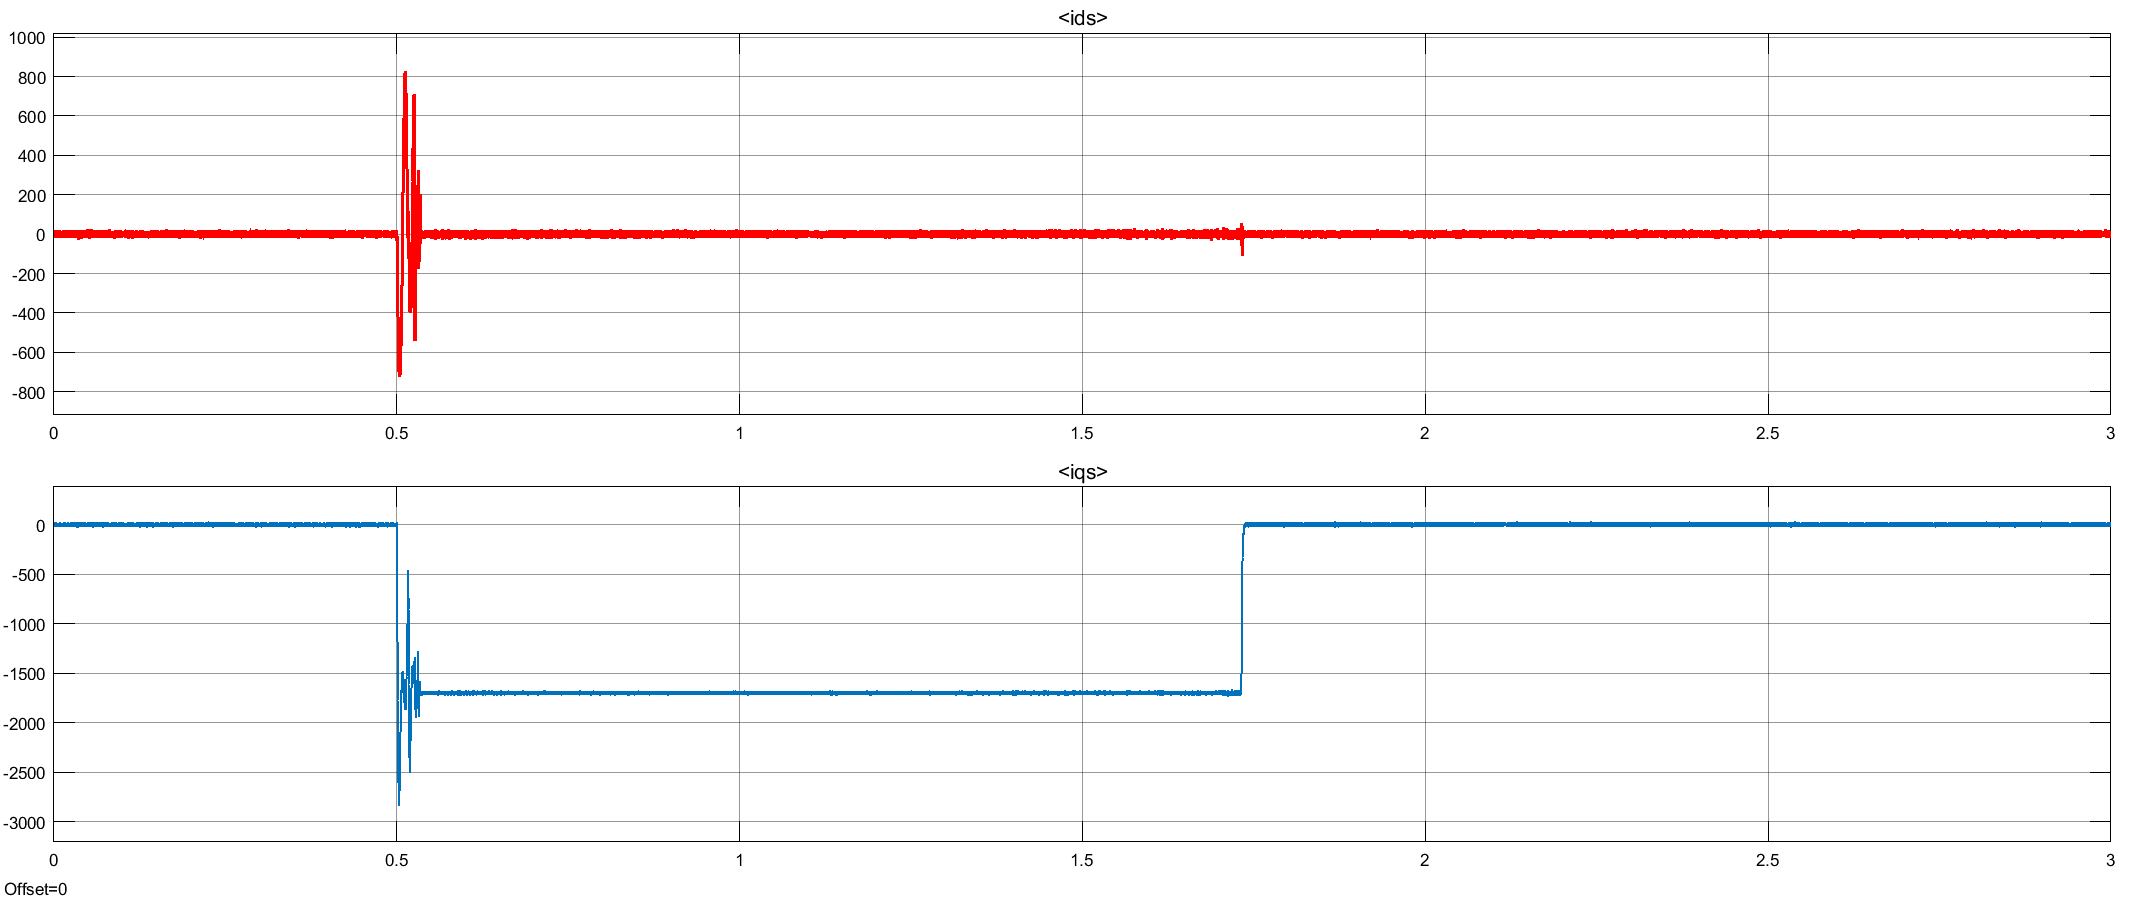
\includegraphics[scale=0.2]{q3_dq.png}
    \caption{Graph of $I_d$ and $I_q$ Currents when Speed Reference is Reversed}
    \label{fig:my_label}
\end{figure}
\textbf{d)}
\begin{figure}[H]
    \centering
    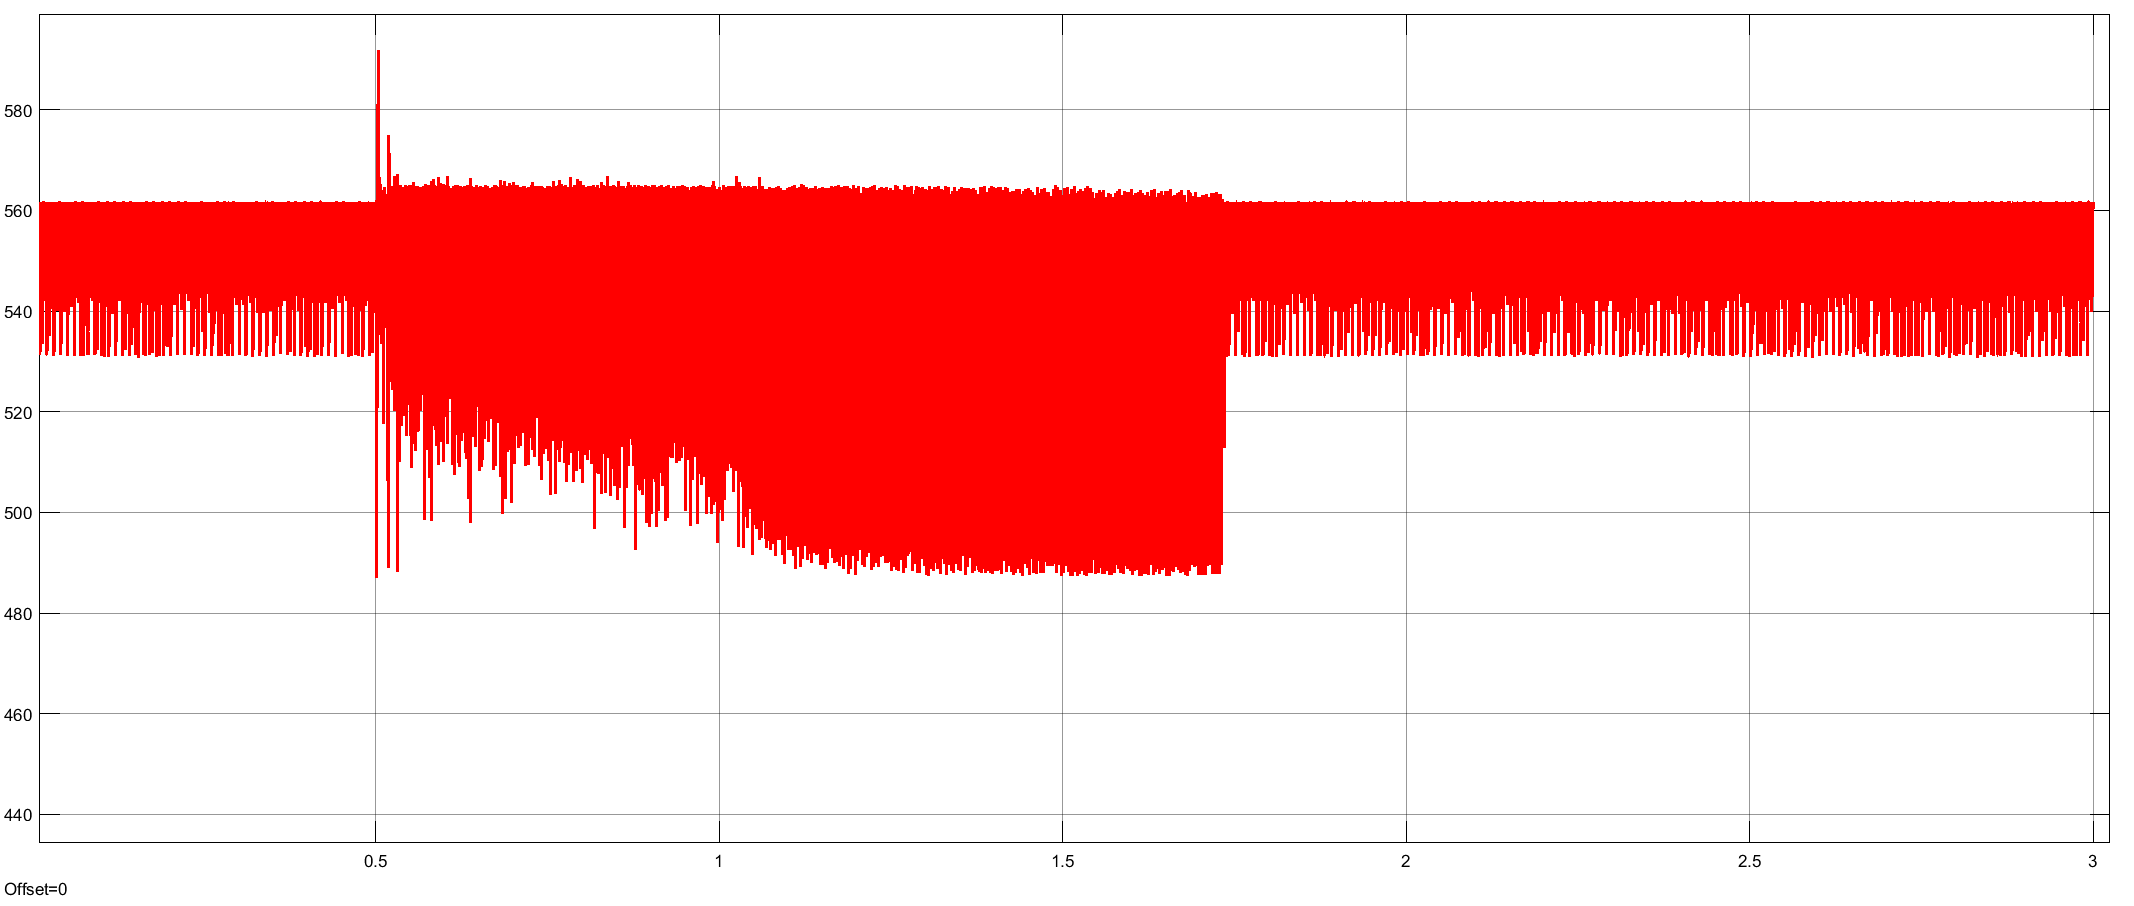
\includegraphics[scale=0.2]{q3_dc.png}
    \caption{Graph of DC Link Voltage when Speed Reference is Reversed}
    \label{fig:my_label}
\end{figure}
\textbf{1.4-} In order to reach high speed values, we may need to get into field weakening, meaning that we need to apply $I_d$ current. To ensure we need to apply $I_d$ current in order to reach 2250 rpm, firstly $I_d$ reference is kept constant at 0 and only speed reference is changed. However, the machine could only go up to slightly higher than 1900 rpm. The speed graph for this case is given below:
\begin{figure}[H]
    \centering
    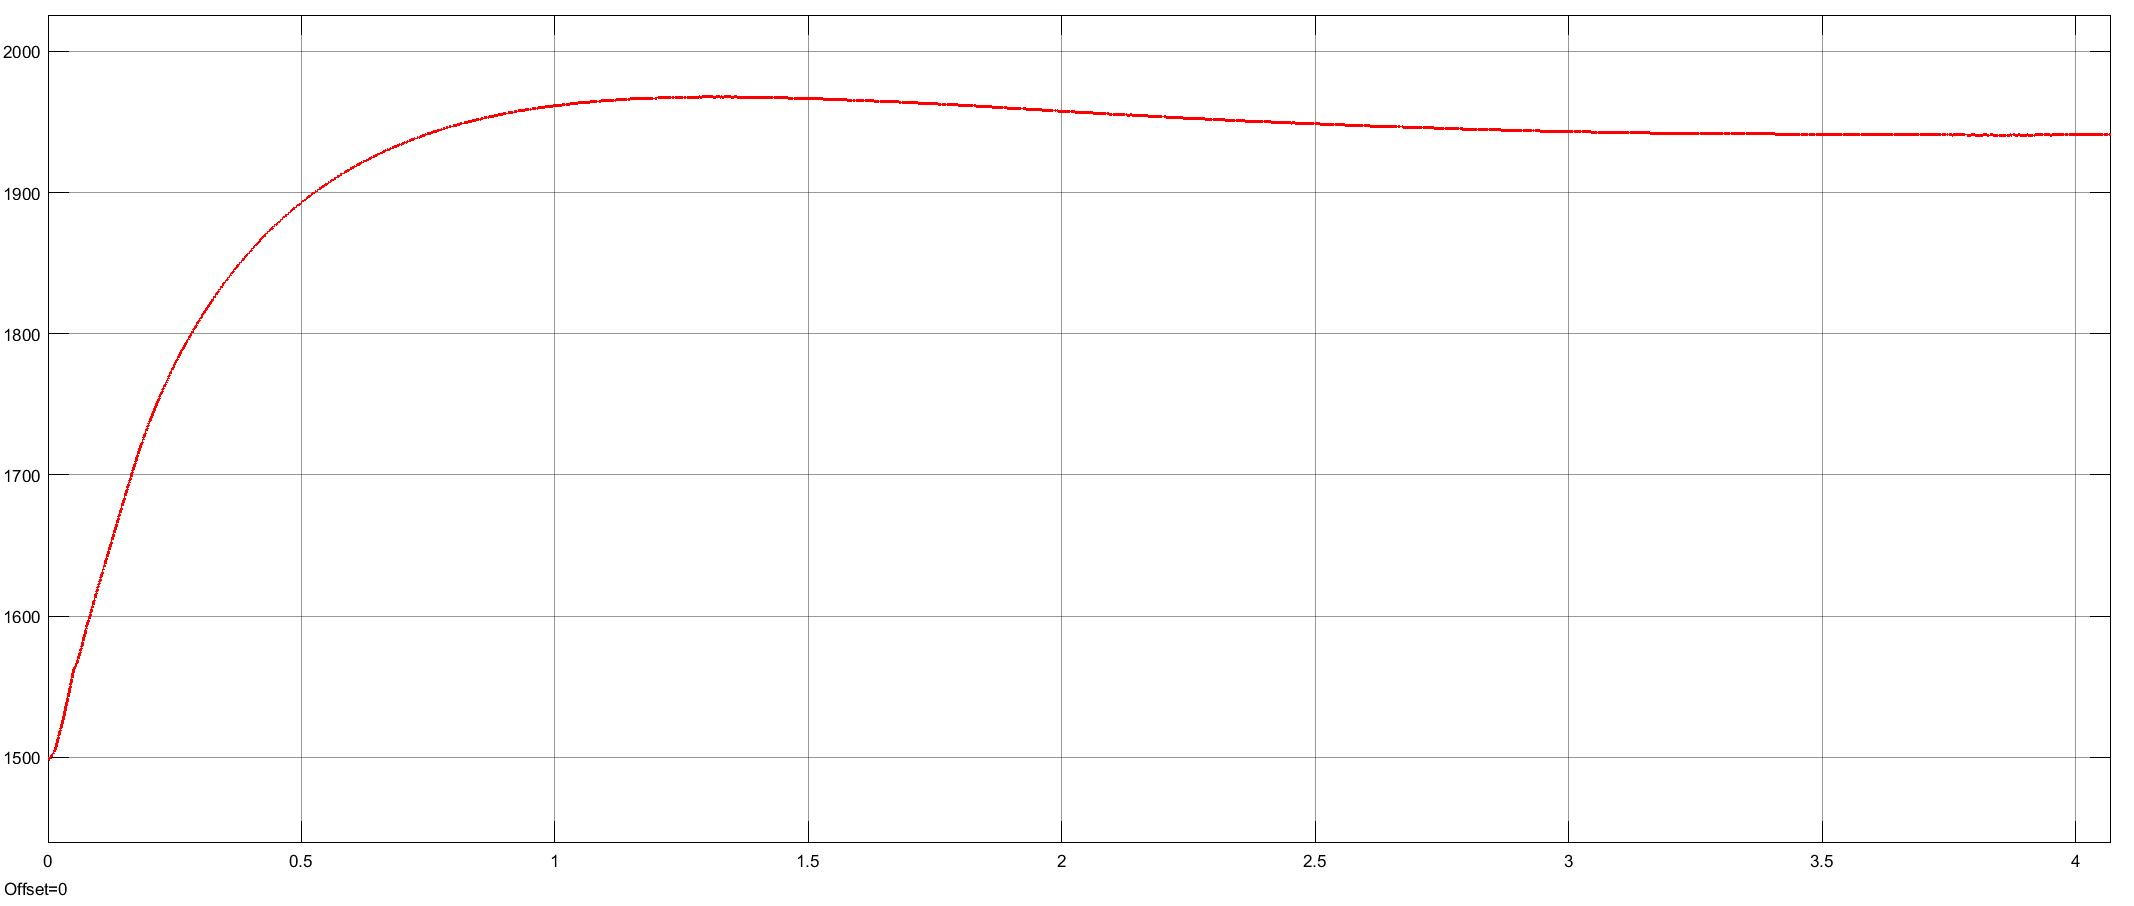
\includegraphics[scale=0.2]{no_dq.png}
    \caption{Graph of Acceleration of the Rotor to 150 \% Speed at no $I_d$ Current}
    \label{fig:my_label}
\end{figure}
As a result, $I_d$ reference value is changed to -360A, so that we can cancel the field created by the magnets in order to achieve higher speeds. The results are given below:
\begin{figure}[H]
    \centering
    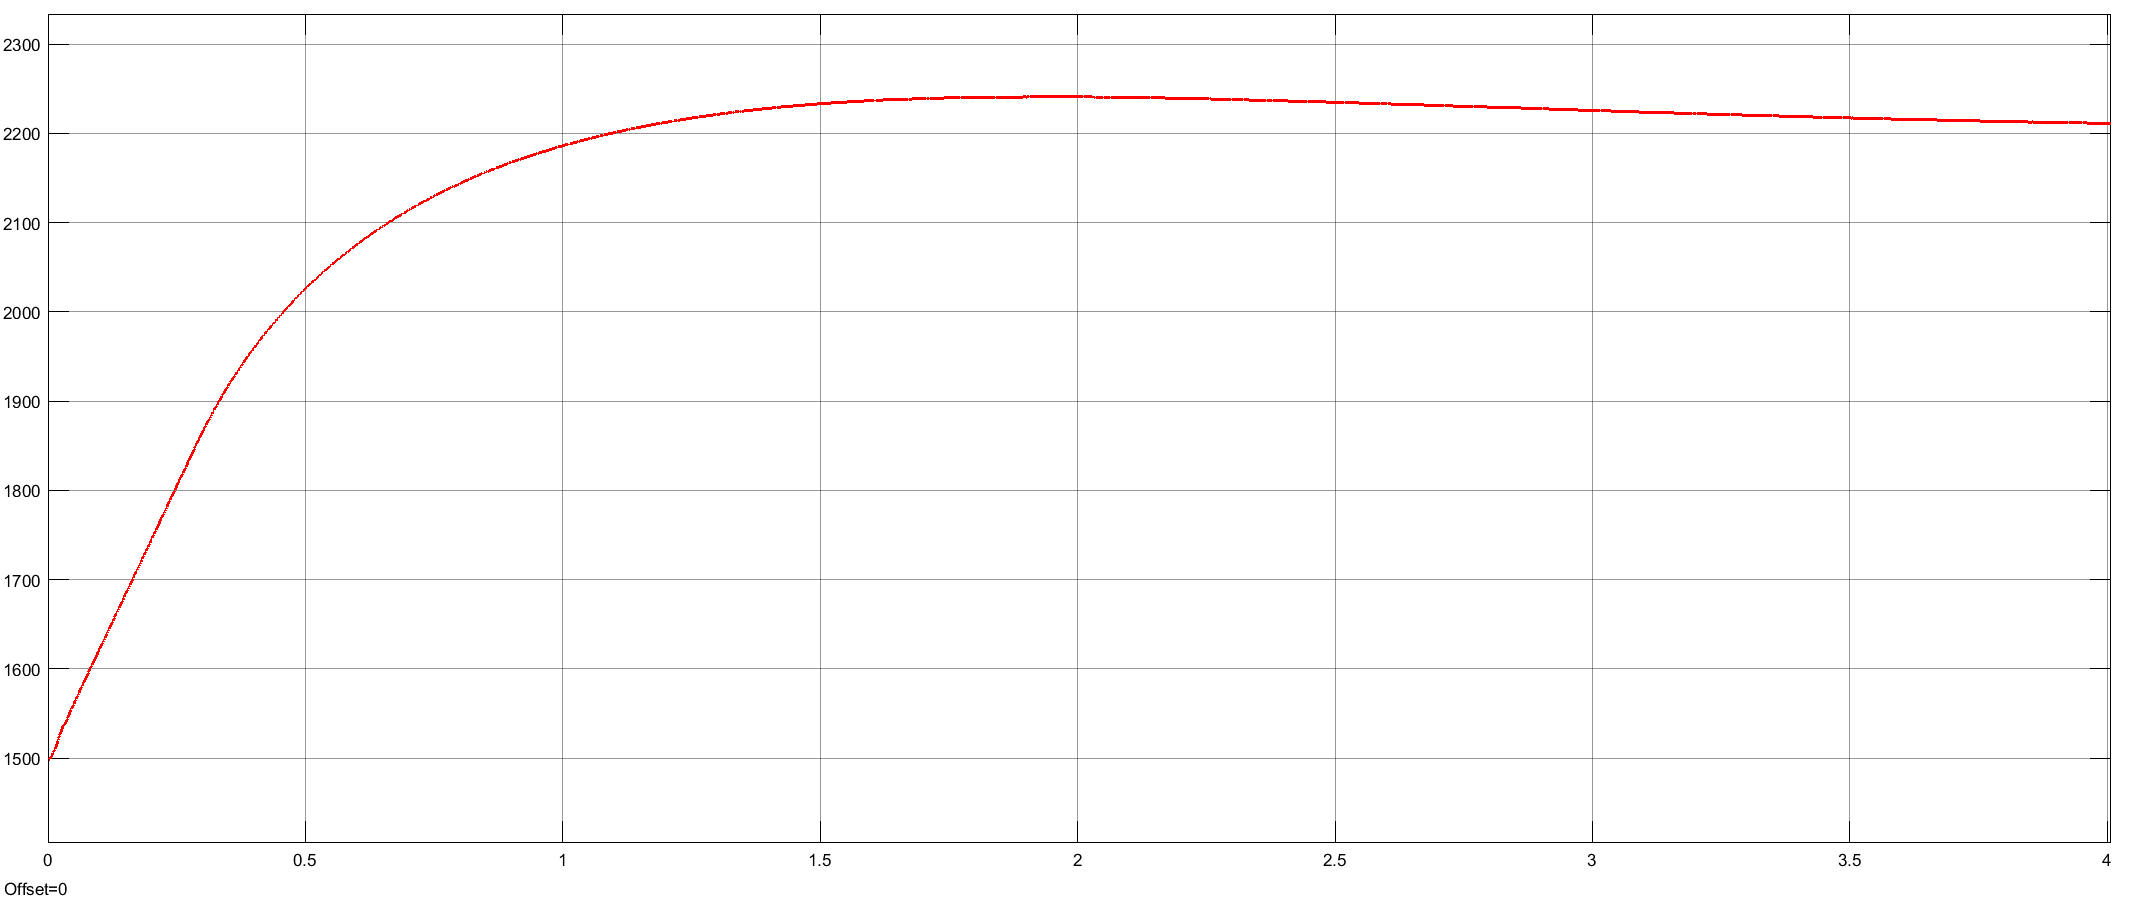
\includegraphics[scale=0.2]{with_dq.png}
    \caption{Graph of Acceleration of the Rotor to 150 \% Speed at -360 Reference $I_d$ Current}
    \label{fig:my_label}
\end{figure}

\begin{figure}[H]
    \centering
    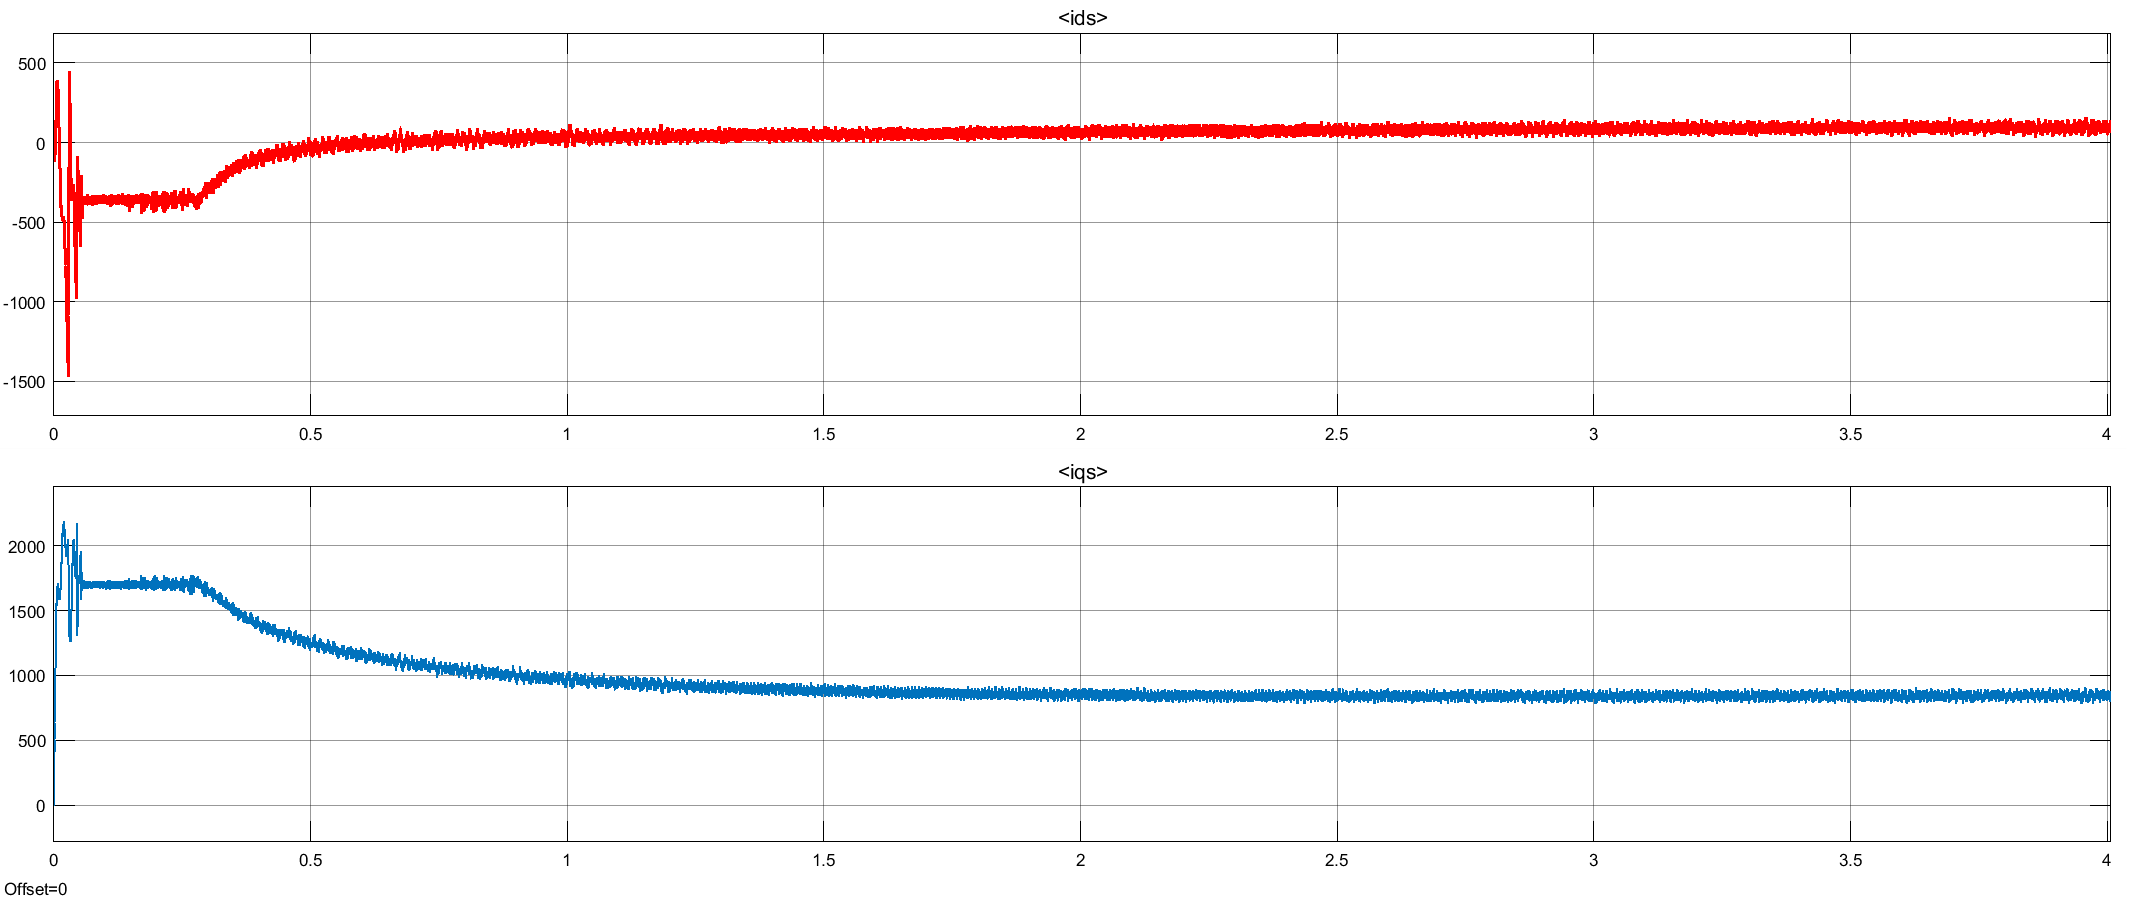
\includegraphics[scale=0.2]{field_weaken.png}
    \caption{Graph of $I_d$ and $I_q$ Currents when the Rotor Accelerates to 150 \% Speed }
    \label{fig:my_label}
\end{figure} \\

\textbf{2-} By using alpha-beta-zero to abc transformation block, reference voltages are obtained in 3-phase reference frame. Result of the reference voltages are given below:
\begin{figure}[H]
    \centering
    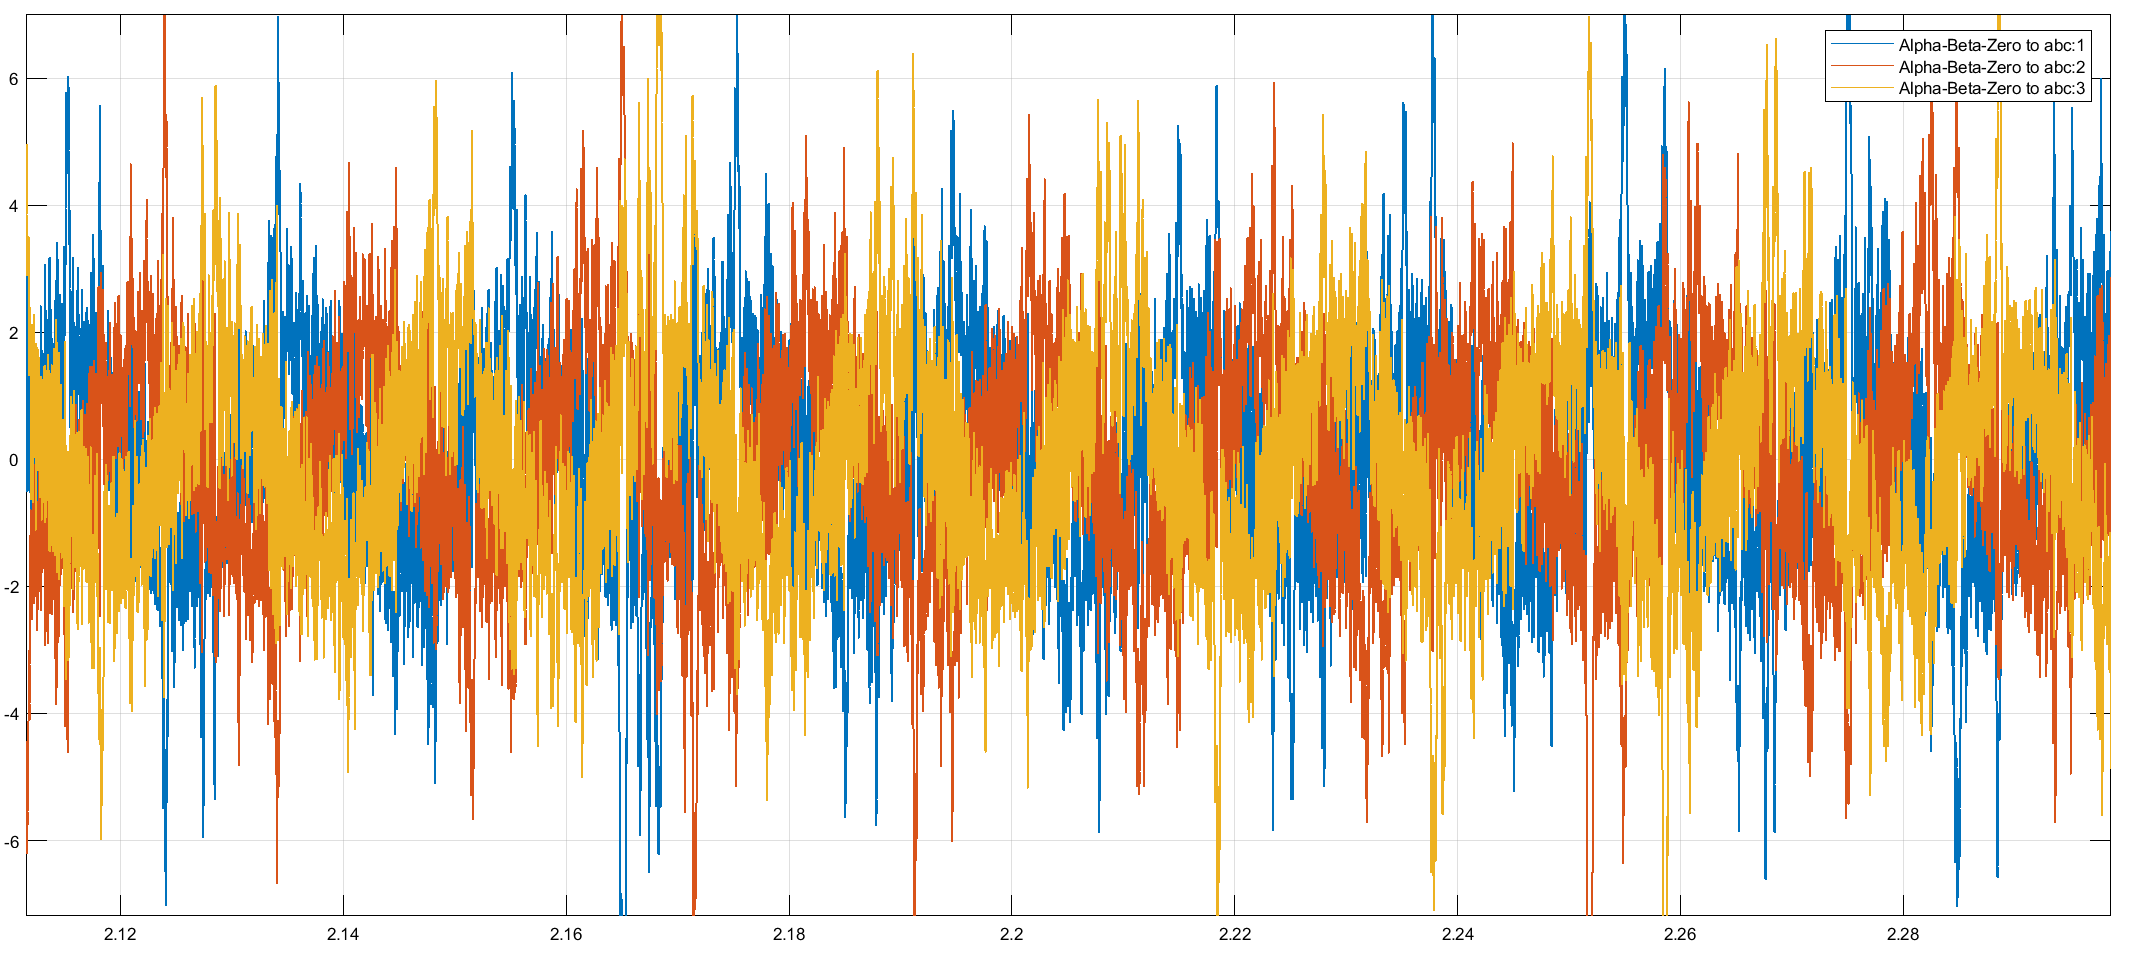
\includegraphics[scale=0.2]{reference_svpwm.png}
    \caption{Graph of Reference Voltages with SVPWM}
    \label{fig:my_label}
\end{figure} \\
Ideally, we expect reference voltages as a sinusoidal waveform which includes 3rd order harmonics as well which enables us to have a higher voltage. Sinusoidal PWM has pure sinusoidal reference voltage waveforms, as expected. FFT analysis output of line current for SVPWM is given below: 
\begin{figure}[H]
    \centering
    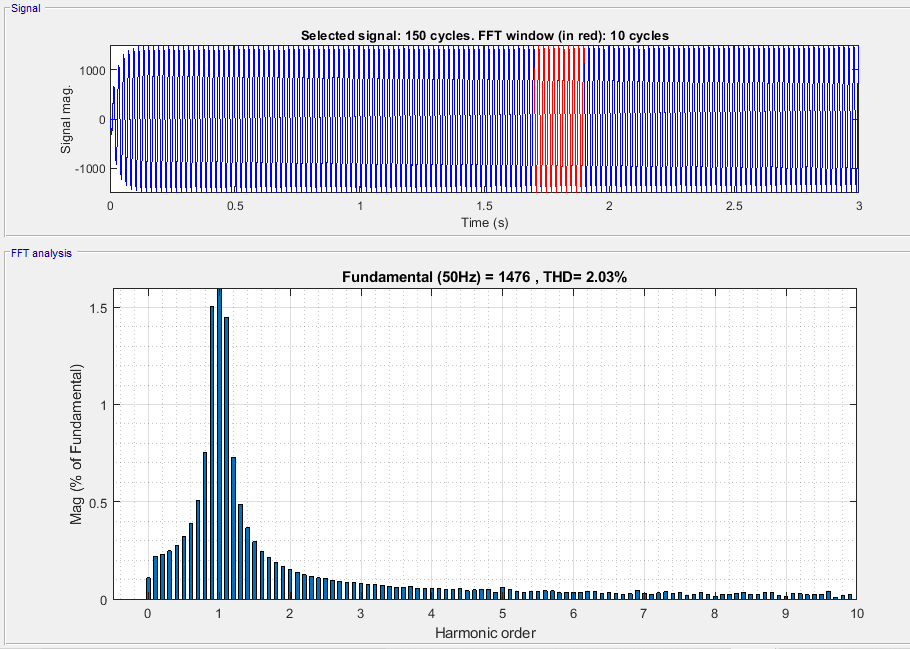
\includegraphics[scale=0.5]{fft.PNG}
    \caption{FFT Analysis of Line Current with SVPWM}
    \label{fig:my_label}
\end{figure} \\
\textbf{3-} SVPWM offers better inverter output quality has less Total Harmonic Distortion than the SPWM. FFT result and THD calculation of SVPWM for rated operation is given below:

\textbf{4-} In SVPWM, duration of zero voltage vectors are always equal to each other, which is the main difference from sinusoidal PWM. It basically shifts reference voltages to make $V_0$ and $V_7$ equal to each other. As a result, SVPWM has 3rd order harmonics in reference voltages, offering higher maximum voltage as indicated above. THD performance of SVPWM is better than SPWM. On the other hand, number of switching is higher in SVPWM, increasing switching losses and reducing efficiency. In addition, SPWM is easier to implement. Hence, sinusoidal PWM can be used for high performance drive since it minimizes switching losses and has better efficiency.
\section{Spent Time for the Project}
Mert Zeybek: 30 hours \\
Canberk Duman: 
\section*{Conclusion}
\tab In this project, we implemented two different techniques for control of the SM-PMSM, sinusoidal PWM and space vector PWM, two of the most widely used PWM techniques. We learned how to implement them on Simulink, observed under different loading and speed conditions for both cases. It was helpful to better understand field oriented control of PMSM devices and it can be helpful if we work in motor control area in our professional engineering careers.
\end{document}